\documentclass[mstat,12pt]{unswthesis}


\newenvironment{CSLReferences}%
  {}%
  {\par}


\usepackage{color}
\usepackage{fancyvrb}
\usepackage{float}
\usepackage{catchfile}
\usepackage{booktabs}
\usepackage{array}
\usepackage{pdflscape}
\usepackage{caption}[hypcap=false]
\usepackage[chapter,nottoc]{tocbibind}

% Configure package settings
\captionsetup[table]{skip=10pt}
\setcounter{secnumdepth}{3} % Ensures sections, subsections, and subsubsections are numbered

\newcommand{\VerbBar}{|}
\newcommand{\VERB}{\Verb[commandchars=\\\{\}]}
\DefineVerbatimEnvironment{Highlighting}{Verbatim}{commandchars=\\\{\}}
% Add ',fontsize=\small' for more characters per line
\usepackage{framed}
\definecolor{shadecolor}{RGB}{248,248,248}
\newenvironment{Shaded}{\begin{snugshade}}{\end{snugshade}}
\newcommand{\AlertTok}[1]{\textcolor[rgb]{0.94,0.16,0.16}{#1}}
\newcommand{\AnnotationTok}[1]{\textcolor[rgb]{0.56,0.35,0.01}{\textbf{\textit{#1}}}}
\newcommand{\AttributeTok}[1]{\textcolor[rgb]{0.77,0.63,0.00}{#1}}
\newcommand{\BaseNTok}[1]{\textcolor[rgb]{0.00,0.00,0.81}{#1}}
\newcommand{\BuiltInTok}[1]{#1}
\newcommand{\CharTok}[1]{\textcolor[rgb]{0.31,0.60,0.02}{#1}}
\newcommand{\CommentTok}[1]{\textcolor[rgb]{0.56,0.35,0.01}{\textit{#1}}}
\newcommand{\CommentVarTok}[1]{\textcolor[rgb]{0.56,0.35,0.01}{\textbf{\textit{#1}}}}
\newcommand{\ConstantTok}[1]{\textcolor[rgb]{0.00,0.00,0.00}{#1}}
\newcommand{\ControlFlowTok}[1]{\textcolor[rgb]{0.13,0.29,0.53}{\textbf{#1}}}
\newcommand{\DataTypeTok}[1]{\textcolor[rgb]{0.13,0.29,0.53}{#1}}
\newcommand{\DecValTok}[1]{\textcolor[rgb]{0.00,0.00,0.81}{#1}}
\newcommand{\DocumentationTok}[1]{\textcolor[rgb]{0.56,0.35,0.01}{\textbf{\textit{#1}}}}
\newcommand{\ErrorTok}[1]{\textcolor[rgb]{0.64,0.00,0.00}{\textbf{#1}}}
\newcommand{\ExtensionTok}[1]{#1}
\newcommand{\FloatTok}[1]{\textcolor[rgb]{0.00,0.00,0.81}{#1}}
\newcommand{\FunctionTok}[1]{\textcolor[rgb]{0.00,0.00,0.00}{#1}}
\newcommand{\ImportTok}[1]{#1}
\newcommand{\InformationTok}[1]{\textcolor[rgb]{0.56,0.35,0.01}{\textbf{\textit{#1}}}}
\newcommand{\KeywordTok}[1]{\textcolor[rgb]{0.13,0.29,0.53}{\textbf{#1}}}
\newcommand{\NormalTok}[1]{#1}
\newcommand{\OperatorTok}[1]{\textcolor[rgb]{0.81,0.36,0.00}{\textbf{#1}}}
\newcommand{\OtherTok}[1]{\textcolor[rgb]{0.56,0.35,0.01}{#1}}
\newcommand{\PreprocessorTok}[1]{\textcolor[rgb]{0.56,0.35,0.01}{\textit{#1}}}
\newcommand{\RegionMarkerTok}[1]{#1}
\newcommand{\SpecialCharTok}[1]{\textcolor[rgb]{0.00,0.00,0.00}{#1}}
\newcommand{\SpecialStringTok}[1]{\textcolor[rgb]{0.31,0.60,0.02}{#1}}
\newcommand{\StringTok}[1]{\textcolor[rgb]{0.31,0.60,0.02}{#1}}
\newcommand{\VariableTok}[1]{\textcolor[rgb]{0.00,0.00,0.00}{#1}}
\newcommand{\VerbatimStringTok}[1]{\textcolor[rgb]{0.31,0.60,0.02}{#1}}
\newcommand{\WarningTok}[1]{\textcolor[rgb]{0.56,0.35,0.01}{\textbf{\textit{#1}}}}




%%%%%%%%%%%%%%%%%%%%%%%%%%%%%%%%%%%%%%%%%%%%%%%%%%%%%%%%%%%%%%%%%%
% 
% OK...Now we get to some actual input.  The first part sets up
% the title etc that will appear on the front page
%
%%%%%%%%%%%%%%%%%%%%%%%%%%%%%%%%%%%%%%%%%%%%%%%%%%%%%%%%%%%%%%%%%

\title{Capstone Project by Group K\\[0.5cm]A Comparison of Uni- and Multivariate Cases of Shallow and Deep Neural Networks for Short-Term Electrical Load Forecasting}

%A Data Science Approach to Forecast Electricity Consumption in New South Wales}

\authornameonly{Doug Smithers (z5135363), Tom Bernstein (z3478832), Daniel Sartor (z5350306). }

\author{\Authornameonly}

\copyrightfalse
\figurespagefalse
\tablespagefalse

%%%%%%%%%%%%%%%%%%%%%%%%%%%%%%%%%%%%%%%%%%%%%%%%%%%%%%%%%%%%%%%%%
%
%  And now the document begins
%  The \beforepreface and \afterpreface commands puts the
%  contents page etc in
%
%%%%%%%%%%%%%%%%%%%%%%%%%%%%%%%%%%%%%%%%%%%%%%%%%%%%%%%%%%%%%%%%%%


%%%%%%%%%%%%%%%%%%%%%%%%%%%%%%%%%%%%%%%%%%%%%%%%%%%%%%%%%%%%%%%%%%%%%%%
%
%  A small sample UNSW Coursework Masters thesis file.
%  Any questions to Ian Doust i.doust@unsw.edu.au and/or Gery Geenens ggeenens@unsw.edu.au
%
%%%%%%%%%%%%%%%%%%%%%%%%%%%%%%%%%%%%%%%%%%%%%%%%%%%%%%%%%%%%%%%%%%%%%%%
%
%  The first part pulls in a UNSW Thesis class file.  This one is
%  slightly nonstandard and has been set up to do a couple of
%  things automatically
%
 
%%%%%%%%%%%%%%%%%
%% Precisely one of the next four lines should be uncommented.
%% Choose the one which matches your degree, uncomment it, and comment out the other two!
%\documentclass[mfin,12pt]{unswthesis}    %%  For Master of Financial Mathematics 
%\documentclass[mmath,12pt]{unswthesis}   %%  For Master of Mathematics
%\documentclass[mstat,12pt]{unswthesis}  %%  For Master of Statistics
%%%%%%%%%%%%%%%%%



\linespread{1}
\usepackage{amsfonts}
\usepackage{amssymb}
\usepackage{amsthm}
\usepackage{latexsym,amsmath}
\usepackage{graphicx}
\usepackage{afterpage}
\usepackage[colorlinks]{hyperref}
 \hypersetup{
     colorlinks=true,
     linkcolor=blue,
     filecolor=blue,
     citecolor= black,      
     urlcolor=cyan,
     }
\usepackage{textcomp}
\usepackage{longtable}
\usepackage{booktabs}
\usepackage{float}

%%%%%%%%%%%%%%%%%%%%%%%%%%%%%%%%%%%%%%%%%%%%%%%%%%%%%%%%%%%%%%%%%
%
%  The following are some simple LaTeX macros to give some
%  commonly used letters in funny fonts. You may need more or less of
%  these
%
\newcommand{\R}{\mathbb{R}}
\newcommand{\Q}{\mathbb{Q}}
\newcommand{\C}{\mathbb{C}}
\newcommand{\N}{\mathbb{N}}
\newcommand{\F}{\mathbb{F}}
\newcommand{\PP}{\mathbb{P}}
\newcommand{\T}{\mathbb{T}}
\newcommand{\Z}{\mathbb{Z}}
\newcommand{\B}{\mathfrak{B}}
\newcommand{\BB}{\mathcal{B}}
\newcommand{\M}{\mathfrak{M}}
\newcommand{\X}{\mathfrak{X}}
\newcommand{\Y}{\mathfrak{Y}}
\newcommand{\CC}{\mathcal{C}}
\newcommand{\E}{\mathbb{E}}
\newcommand{\cP}{\mathcal{P}}
\newcommand{\cS}{\mathcal{S}}
\newcommand{\A}{\mathcal{A}}
\newcommand{\ZZ}{\mathcal{Z}}
%%%%%%%%%%%%%%%%%%%%%%%%%%%%%%%%%%%%%%%%%%%%%%%%%%%%%%%%%%%%%%%%%%%%%
%
% The following are much more esoteric commands that I have left in
% so that this file still processes. Use or delete as you see fit
%
\newcommand{\bv}[1]{\mbox{BV($#1$)}}
\newcommand{\comb}[2]{\left(\!\!\!\begin{array}{c}#1\\#2\end{array}\!\!\!\right)
}
\newcommand{\Lat}{{\rm Lat}}
\newcommand{\var}{\mathop{\rm var}}
\newcommand{\Pt}{{\mathcal P}}
\def\tr(#1){{\rm trace}(#1)}
\def\Exp(#1){{\mathbb E}(#1)}
\def\Exps(#1){{\mathbb E}\sparen(#1)}
\newcommand{\floor}[1]{\left\lfloor #1 \right\rfloor}
\newcommand{\ceil}[1]{\left\lceil #1 \right\rceil}
\newcommand{\hatt}[1]{\widehat #1}
\newcommand{\modeq}[3]{#1 \equiv #2 \,(\text{mod}\, #3)}
\newcommand{\rmod}{\,\mathrm{mod}\,}
\newcommand{\p}{\hphantom{+}}
\newcommand{\vect}[1]{\mbox{\boldmath $ #1 $}}
\newcommand{\reff}[2]{\ref{#1}.\ref{#2}}
\newcommand{\psum}[2]{\sum_{#1}^{#2}\!\!\!'\,\,}
\newcommand{\bin}[2]{\left( \begin{array}{@{}c@{}}
				#1 \\ #2
			\end{array}\right)	}
%
%  Macros - some of these are in plain TeX (gasp!)
%
\newcommand{\be}{($\beta$)}
\newcommand{\eqp}{\mathrel{{=}_p}}
\newcommand{\ltp}{\mathrel{{\prec}_p}}
\newcommand{\lep}{\mathrel{{\preceq}_p}}
\def\brack#1{\left \{ #1 \right \}}
\def\bul{$\bullet$\ }
\def\cl{{\rm cl}}
\let\del=\partial
\def\enditem{\par\smallskip\noindent}
\def\implies{\Rightarrow}
\def\inpr#1,#2{\t \hbox{\langle #1 , #2 \rangle} \t}
\def\ip<#1,#2>{\langle #1,#2 \rangle}
\def\lp{\ell^p}
\def\maxb#1{\max \brack{#1}}
\def\minb#1{\min \brack{#1}}
\def\mod#1{\left \vert #1 \right \vert}
\def\norm#1{\left \Vert #1 \right \Vert}
\def\paren(#1){\left( #1 \right)}
\def\qed{\hfill \hbox{$\Box$} \smallskip}
\def\sbrack#1{\Bigl \{ #1 \Bigr \} }
\def\ssbrack#1{ \{ #1 \} }
\def\smod#1{\Bigl \vert #1 \Bigr \vert}
\def\smmod#1{\bigl \vert #1 \bigr \vert}
\def\ssmod#1{\vert #1 \vert}
\def\sspmod#1{\vert\, #1 \, \vert}
\def\snorm#1{\Bigl \Vert #1 \Bigr \Vert}
\def\ssnorm#1{\Vert #1 \Vert}
\def\sparen(#1){\Bigl ( #1 \Bigr )}

\newcommand\blankpage{%
    \null
    \thispagestyle{empty}%
    \addtocounter{page}{-1}%
    \newpage}

%%%%%%%%%%%%%%%%%%%%%%%%%%%%%%%
%
% These environments allow you to get nice numbered headings
%  for your Theorems, Definitions etc.  
%
%  Environments
%
%%%%%%%%%%%%%%%%%%%%%%%%%%%%%%%

\newtheorem{theorem}{Theorem}[section]
\newtheorem{lemma}[theorem]{Lemma}
\newtheorem{proposition}[theorem]{Proposition}
\newtheorem{corollary}[theorem]{Corollary}
\newtheorem{conjecture}[theorem]{Conjecture}
\newtheorem{definition}[theorem]{Definition}
\newtheorem{example}[theorem]{Example}
\newtheorem{remark}[theorem]{Remark}
\newtheorem{question}[theorem]{Question}
\newtheorem{notation}[theorem]{Notation}
\numberwithin{equation}{section}

%%%%%%%%%%%%%%%%%%%%%%%%%%%%%%%%%%%%%%%%%%%%%%%%%%%%%%%%%%%%%%%%%%
%
%  If you've got some funny special words that LaTeX might not
% hyphenate properly, you can give it a helping hand:
%

\hyphenation{Mar-cin-kie-wicz Rade-macher}


\newlength{\cslhangindent}
\setlength{\cslhangindent}{1.5em}
\newlength{\csllabelwidth}
\setlength{\csllabelwidth}{3em}
\newenvironment{CSLReferences}[2] % #1 hanging-ident, #2 entry spacing
 {% don't indent paragraphs
  \setlength{\parindent}{0pt}
  % turn on hanging indent if param 1 is 1
  \ifodd #1 \everypar{\setlength{\hangindent}{\cslhangindent}}\ignorespaces\fi
  % set entry spacing
  \ifnum #2 > 0
  \setlength{\parskip}{#2\baselineskip}
  \fi
 }%
 {}
\usepackage{calc} % for \widthof, \maxof
\newcommand{\CSLBlock}[1]{#1\hfill\break}
\newcommand{\CSLLeftMargin}[1]{\parbox[t]{\maxof{\widthof{#1}}{\csllabelwidth}}{#1}}
\newcommand{\CSLRightInline}[1]{\parbox[t]{\linewidth}{#1}}
\newcommand{\CSLIndent}[1]{\hspace{\cslhangindent}#1}

\bibliographystyle{elsarticle-num}




\begin{document}

\beforepreface

%\afterpage{\blankpage}

% plagiarism

\prefacesection{Plagiarism statement}

\vskip 2pc \noindent I declare that this thesis is my
own work, except where acknowledged, and has not been submitted for
academic credit elsewhere. 

\vskip 2pc  \noindent I acknowledge that the assessor of this
thesis may, for the purpose of assessing it:
\begin{itemize}
\item Reproduce it and provide a copy to another member of the University; and/or,
\item Communicate a copy of it to a plagiarism checking service (which may then retain a copy of it on its database for the purpose of future plagiarism checking).
\end{itemize}

\vskip 2pc \noindent I certify that I have read and understood the University Rules in
respect of Student Academic Misconduct, and am aware of any potential plagiarism penalties which may 
apply.\vspace{24pt}

\vskip 2pc \noindent By signing 
this declaration I am
agreeing to the statements and conditions above.
\vskip 2pc \noindent
\begin{figure}[H]
    \centering
    \includegraphics[width=1.0\linewidth]{tb_signature.png}
\end{figure}
%Signed: \rule{7cm}{0.25pt} \hfill Date: \rule{4cm}{0.25pt} \\[1cm]
Signed: \rule{7cm}{0.25pt} \hfill Date: \rule{4cm}{0.25pt} \\[1cm]
Signed: \rule{7cm}{0.25pt} \hfill Date: \rule{4cm}{0.25pt} \\[1cm]
\vskip 1pc

%\afterpage{\blankpage}

% Acknowledgements are optional


% \prefacesection{Acknowledgements}
% 
% {\bigskip}By far the greatest thanks must go to my supervisor for the
% guidance, care and support they provided.\\[1cm] Thanks must also go to
% Emily, Michelle, John and Alex who helped by proof-reading the document
% in the final stages of preparation.\\[1cm] Although I have not lived
% with them for a number of years, my family also deserve many thanks for
% their encouragement. Thanks go to Robert Taggart for allowing his thesis
% style to be shamelessly copied.\\[1cm] 
% 
% {\bigskip\bigskip\bigskip\noindent} 25/07/2020.
% 
% %\afterpage{\blankpage}

% Abstract

\prefacesection{Abstract}

%The image below gives you some hint about how to write a good abstract.

\par

%\bigskip \includegraphics[width=10cm,height=10cm]{good-abstract.png}

%\afterpage{\blankpage}

Forecasting electrical load is critical for electricity generators and distributors to efficiently dispatch the load, schedule energy transfers, and plan contingencies. Accurate forecasting can significantly lower operational costs, prevent outages, and reduce emissions. Short-term load forecasting (STLF), over a 1-24 hour period, is imperative in managing operations, and STLF will be the focus of this study. Many techniques have been applied to this task. However, the application of neural networks (NNs) is salient, as they do not require the estimation of a complex load model and, crucially, have shown superior forecast accuracy compared to other methods. Since their first use in the late 1980s, advances in NN architectures have offered improved performance and prediction accuracy. This study will compare a simple feed-forward Muli-Layer Perceptron (MLP) NN to a more complex architecture in the Bi-Directional Long Short-Term Memory (BD-LSTM) network to assess the performance gains that come with these advances. In addition, a univariate model will be compared to a multivariate model for each architecture to assess the impact of including additional features. Finally, the model depth of each architecture will be increased to see if performance gains come from allowing the models to find more complex relationships between attributes. While increasing model complexity may come with performance gains, it will also come with increased computational load, which will also be examined. The model results will be compared to predictions by a model supplied by the AEMO Market Management System, which will be used as a baseline for performance. The results from this study have shown that the increased training time required for the complex models prevented them from outperforming the simple MLPs in the timeframe of this project, and more time must be given to training to come to a definitive conclusion. Multivariate models were shown to outperform their univariate equivalents on greater prediction horizons, with the added attributes providing more information for the models to learn relationships. The results showed no clear benefit from increasing model depth. Finally, the results could not match those from the baseline model, and more testing is needed for the applied models to be competitive.


\afterpreface





%%%%%%%%%%%%%%%%%%%%%%%%%%%%%%%%%%%%%%%%%%%%%%%%%%%%%%%%%%%%%%%%%%
%
% Now we can start on the first chapter
% Within chapters we have sections, subsections and so forth
%
%%%%%%%%%%%%%%%%%%%%%%%%%%%%%%%%%%%%%%%%%%%%%%%%%%%%%%%%%%%%%%%%%%



%%%%%%%%%%%%%%%%%%%%%%%%%%%%%%%%%%%%%

%\afterpage{\blankpage}


\hypertarget{introduction}{%
\chapter{Introduction}\label{introduction}}

Forecasting electrical load, typically performed over short- (1-24 hours), medium- (1 day to several months), and long-term prediction horizons (more than a full year ahead) \cite{Yalcinoz2005}, is critical for electricity generators and distributors \cite{Djukanovic1995}\cite{Berk2018}. These stakeholders are particularly reliant on short-term load forecasts (STLF), which are essential for daily operations, and accurate short-term forecasting is required to enable efficient load dispatching, energy transfer scheduling, and contingency planning and has the potential to significantly lower operational costs, prevent outages, improve safety and reduce emissions \cite{KavousiFard2014}\cite{Dong2021}. Therefore, STLF will be the focus of this study.

Load forecasting techniques, both quantitative and qualitative, are typically classified into three major groups: traditional forecasting, modified traditional forecasting, and soft computing techniques \cite{Singh2013}. Neural networks (NN), classified as a soft computing technique, have shown to have significant advantages over other methods because they do not require a load model, are not reliant on a functional form of a forecast model, and, importantly, can produce higher forecast accuracy \cite{Djukanovic1995}. The advantages presented by utilising NNs for STLF, along with the data science expertise of the team, have led to the decision to focus on this class of models for this project.

Models may be classified as univariate, taking only previous load observations as inputs, or multivariate (i.e. causal), where the load is modelled as a function of other exogenous variables, such as weather or social variables \cite{Hippert2001}. Demand on the electricity grid strongly correlates to the weather, with variables such as temperature, relative humidity, dew point, dry bulb temperature, wind speed and cloud cover commonly used \cite{Raza2015}. However, several models have produced high accuracy using only temperature, as these weather attributes have high multicollinearity \cite{Chandra2021}. For short-term load forecasting, as weather variables change smoothly over time, univariate models are generally sufficient, with multivariate models often considered impractical due to their increased computational load \cite{ElHawary2017}. The intermittent nature of renewable energy feeding into the grid, particularly wind and solar, is a challenge when producing an STLF \cite{Hoori2019}. Therefore, wind and solar radiance observations could influence the model's effectiveness. This project is an excellent opportunity to understand the impact of adding exogenous features for STLF models.

Along with a ten-year load dataset across four Australian states, temperature observations over the same period are available. Temperature varies dramatically across each state, and data from only a single station in each state is available. The absence of data from other locations is a potential limitation of this project. However, the relative change in temperature across the day may be sufficiently well correlated with weather stations across each state. 

Numerous other features can be engineered from the available data, which may add value to the models. For example, the classification of work or non-work days and an attribute for the hour of the day may prove useful. In addition, there is a strong correlation between load values for each time step and for the prior hour or the same hour in the previous week \cite{Raza2015}, and these values can be used as input.

Simple feed-forward NNs have been used for time-series forecasting since the late 1980s \cite{Czernichow1996}, with many advancements made since then. This study will offer an opportunity to examine the advantages of these recent developments. This paper will compare a set of feed-forward NNs to a set of more complex bi-directional long short-term memory (BD-LSTM) models. The LSTM model is a variant of the Recurrent NN (RNN), which uses recurrent connections to a context layer, allowing the network to have memory of previous inputs. While traditional RNNs suffer from two significant issues, exploding and vanishing gradients, LSTM networks are a modification of RNNs, employing memory cells to control the gradient flow, allowing them to overcome these problems. The BD-LSTM extends this concept further and uses two separate context layers, allowing information to flow backward and forward at each time step \cite{Chandra2021}. 

For each of these architectures, we will compare shallow networks to deeper networks and univariate models to multivariate, giving eight models in total. The aim will be to determine the gains in prediction accuracy that come with increasing model depth and the number of input features. While increased complexity may improve performance, it will also add computational load and, consequently, extend the required training time. These aspects will also be examined here. We will compare the results of each model to a set of predictions from a model created by the AEMO Market Management System. While no specific details on this model were supplied, the results from this model will serve as a baseline to measure predictive performance.

The rest of the paper is organised as follows. Chapter \ref{literature-review} presents a literature review of previous work. Chapter \ref{material-and-methods} details the materials and methods used. Chapter \ref{exploratory-data-analysis} details the exploratory data analysis. Chapter \ref{analysis-and-results} presents the analysis and results. Chapter \ref{discussion} provides a discussion of results, and Chapter \ref{conclusion-and-further-issues} concludes the study and recommends further actions.
\hypertarget{literature-review}{%
\chapter{Literature Review}\label{literature-review}}

%Here are a few references that can be useful: (Xie et al., 2018) and
%(Lafaye de Micheaux et al., 2013). See also
%\url{https://bookdown.org/yihui/rmarkdown-cookbook/}

\section{Pre-Processing and Feature Engineering} \label{Pre-Processing and Feature Engineering}
How features are coded influences an NN's ability to map inputs to outputs and affects the way it learns \cite{Dudek2019}. Two main properties have an impact. The first is the adjacency property, which dictates that adjacent values in the original space should be represented by adjacent values in the code space. The second is periodicity, which says that the starting and ending values in the original space should have similar values in the code space. As an example, \cite{Yazici2022} used a polar coordinate system to represent the hour-of-day parameter using Equation \ref{hour-func}, where $h$ is the new feature vector corresponding to hour of the day, $t$ is the hour of the day (from 1 to 24) and $c$ is the total number of hours in the day. For any feature engineering for this project, these principles will be adhered to, where applicable.

\begin{equation}\label{hour-func}
    h = \sin \left(\frac{2\pi t}{c} \right)
\end{equation}

Four components affect a time series: trends, cyclical variations, seasonal variations and random variation. A comparison of several artificial intelligence-based STLF techniques \cite{Raza2015} identified additional features that could be engineered from input data that contains only hourly temperature, similar to the data supplied for this project. As the load heavily correlates with temperature, it is subject to seasonal variations. Seasonally clustering the observations was shown to improve model performance in this study.

Additionally, the load profile over each hour through each day of the week, which directly relates to human activity, was also examined in \cite{Raza2015}.\footnote{This relationship appears in our data and is presented in Section \ref{exploratory-data-analysis}} \cite{Raza2015} showed a repeating pattern of high use on weekends. This pattern will vary greatly depending on the part of the world from which and the season during which the data are sourced. It is important to consider this in our project, and it may be beneficial to include an attribute classifying the day of the week or a classification of working days. It may also be beneficial to consider non-typical days, such as special events or public holidays. Further, \cite{Raza2015} detailed the high autocorrelation with previous load data and noted that previous observations (e.g., the load observation for the previous hour or the same hour in the previous week) are useful predictors. 

\section{Neural Networks}
When comparing NN architectures, deep learning techniques have been shown to have advantages over shallow techniques, with superior generalisation and accuracy, but often at the expense of computational cost due to their complex network structure \cite{Dong2021}. Of the many deep learning techniques applied across the vast spectrum of data modelling, Long short-term memory (LSTM), a type of Recurrent NN (RNN) and Gated Recurrent Unit (GRU) have gained popularity for time-series problems due to their efficient feature extraction and high prediction performances \cite{Yazici2022}. Of the variants of LSTM architectures, bi-directional LSTM networks have been compared favourably to other methods \cite{Chandra2021}\cite{Wang2019}. Another promising, although lesser studied, technique is the One-Dimensional Convolutional Neural Network (1D-CNN), which alleviates the issue of long RNN training times through the use of causal convolutional layers, with no recurrent connections \cite{Yazici2022}.

\subsection{Hyperparameter Tuning}
The authors in \cite{Raza2015} found that the predictive performance of a neural network was heavily dependent on the chosen activation functions and training algorithms. As there is no general rule for choosing these parameters, it will be essential to ensure that they are well-researched for each of the applied model architectures, and experimentation will be required to achieve the optimal result.

A comprehensive guide to hyperparameter (learning rate, batch size, momentum and weight decay) tuning is given in \cite{Smith2018}, which pays particular attention to the examination of training validation and test loss curves for evidence of under- or over-fitting. The goal of training should be to obtain maximum performance while minimising computation time. The study showed that optimal architecture and hyperparameter settings could be determined in the early stages of training, saving the need for a grid or random search, which is computationally expensive. The article implements the techniques of Cyclical Learning Rates (CLR) and Learning Rate Range Testing (LRRT), first introduced in \cite{Smith2015} and then revised in \cite{Smith2017}. 

CLR involves specifying a lower and upper bound for the learning rate and a step size. For each cycle, the learning rate is linearly increased from the lower to the upper bound and then linearly back down again. The LRRT involves starting training with a small learning rate and slowly increasing it linearly in a pre-training run. This process allows for determining how well the network trains over a range of learning rates to find the maximum learning rate that provides stable training. This value will be used as the upper bound of the CLR. The minimum learning rate is often chosen to be a factor of 3 to 4 times less than the maximum. Using large learning rates with CLR allows the network to reach super-convergence \cite{SmithTopin2019} (i.e. minimisation of loss over a few iterations). Further, \cite{Smith2017} propose a modification of CLR, dubbed \textit{1cycle}, where one cycle is smaller than the total number of epochs, allowing the learning rate to decrease below the initial rate for the final iterations.

The author in \cite{Smith2017} showed that, along with large learning rates, other regularisation techniques, such as small batch sizes, weight decay and dropout, must be balanced for each dataset and architecture. In particular, small weight decay values (below $10^{-4}$) must be used in concert with large learning rates. The weight decay value should remain constant throughout training. The article suggests using large batch sizes, which allow large learning rates when using \textit{1cycle}. Larger momentum values will speed up training and help the network escape saddle points but can impact final convergence. A test of values between 0.9 and 0.99 should be performed, with the best value set as a constant.

\subsection{Simple Networks}
\subsubsection{Feed-Forward Neural Networks}
Neural networks have become a popular option for STLF due to their ability to model complex and non-linear relationships, which are challenging for conventional techniques. A simple feed-forward NN consisting of an input layer, a single hidden layer containing a finite number of hidden neurons, and an output layer has the power to act as a universal approximator, regardless of the chosen activation function \cite{Csaji2001}\cite{Gasparin2021}. That is, no matter the complexity of the function being modelled, the NN can approximate it. In multi-step-ahead forecasting, the dimension of the output layer relates to the forecasting horizon. Feed-forward NNs have been implemented for time-series problems since the late 1980s and early 1990s \cite{Czernichow1996}. 

In \cite{Park1991}, the authors propose an NN with a single hidden layer to forecast 24 hours ahead using load and temperature data as input. \cite{Srinivasan1994} presents one of the original applications of a feed-forward NN in producing hourly load forecasts. In a comparison of many early studies using feed-forward NNs for STLF, \cite{Hippert2001} found that a single hidden layer was sufficient in most applications. Most networks compared in this study utilised sigmoidal activation functions for the hidden layers and a linear function for the output layer to give the predicted output. In \cite{Mohammad2018}, a comparison of deep feed-forward NNs was performed, with one case using tanh activation functions for the hidden layers and the other using sigmoid, with the former providing better prediction accuracy. For a simple feed-forward MLP network, \cite{Dudek2013} first applied a local learning technique designed to take into account the differences in input and output spaces caused by seasonal or cyclical variations, reported that the use of a single hidden neuron with a sigmoid activation function produced comparable results to models with larger numbers of hidden neurons. It is noted that the simplification of the network with local training may be required to achieve such results with such simple model architectures. For feed-forward NN models, the use of the Adam optimiser, which adapts the learning rate for each parameter as the learning progresses, has been regularly used \cite{Chandra2021}\cite{Gasparin2021}\cite{Chen2018} and has been shown to as having superior performance to stochastic gradient descent, which retains consistent gradients throughout training \cite{Hippert2001}.

More recently, advances in NN architectures have seen more complex feed-forward models applied to STLF. For example,  \cite{Chen2018} used an approach inspired by deep Residual Networks (ResNets) to predict day-ahead forecasts using a much deeper architecture than the models mentioned above. \cite{Hinton2006} introduced the Deep Belief Network (DBN), which is composed of stacked layers of Restricted Boltzmann Machines (RBMs), which address the problems of slow learning and training becoming stuck in local minima.

\subsection{Deep Networks}
\subsubsection{Long Short-Term Memory Networks}
Simple Recurrent Neural Networks (RNNs) use time series data. They are commonly used for temporal problems and utilise a context layer that enables the network to have memory of prior inputs, which influences the current input and output. This memory allows them to extract time-varying patterns in data \cite{Hewamalage2020}. However, RNNs can suffer from two well-known problems: exploding gradients and vanishing gradients. Vanishing gradients occur when the gradient becomes so small that the weight parameters update until they become insignificant (i.e. 0), stopping the network from learning. Conversely, when the gradients grow too large, the model weights explode, making the model unstable. Long Short-Term Memory (LSTM) models, first introduced in \cite{Hochreiter1997}, were developed to overcome these problems. They maintain the same topological structure as an Elman RNN (a common type of simple RNN). However, the network's inner cells' composition differs \cite{Gasparin2021}. Each cell implements a gated system, allowing the control of gradient flow.

The Bi-Directional LSTM (BD-LSTM) further develops this concept and uses two context layers, allowing information to proceed forward and backward through the network. Inputs are read from two directions, one from past to future and the other from future to past. This allows the network to preserve information from both the past and future at any point in time, giving it a long-range context. The BD-LSTM network structure used by \cite{Chandra2021} is given in \ref{BDLSTM}, with the LSTM cell composition shown in \ref{LSTMcell}.

\begin{figure}[H]
    \centering
    \includegraphics[width=0.75\linewidth]{Final Report//Figures/image.png}
    \caption{The BD-LSTM network structure \cite{Chandra2021}.}
    \label{BDLSTM}
\end{figure}

\begin{figure}[H]
    \centering
    \includegraphics[width=0.75\linewidth]{Final Report//Figures/LSTM-cell.png}
    \caption{The composition of a LSTM cell, as depicted in \cite{Chandra2021}}
    \label{LSTMcell}
\end{figure}

In \cite{Din2017}, an RNN was shown to have less error than a feed-forward NN on all metrics and all domains. In \cite{Chandra2021}, a comparison of shallow and deep learning techniques for STLF was performed, including three variants of LSTM models: traditional LSTM, BD-LSTM,  and Encoder-Decoder LSTM (ED-LSTM), as well as a One-Dimensional Convolutional Neural Network (1D-CNN). LSTM networks utilise memory cells and gates, allowing long-term dependencies to be better captured in temporal sequences. Simple RNNs have limited ability to learn long-term dependencies and can suffer from the issue of vanishing or exploding gradients. Therefore, LSTM models, which are variants of RNNs, are advantageous for STLF. This study's three LSTM models outperformed shallow learning models and simple RNNs, with ED-LTSM and BD-LTSM giving the best results. 

For this project, we decided to study a variety of NN architectures rather than multiple versions of the same principle. Therefore, the BD-LSTM method, first introduced in \cite{Schuster1997}, will be investigated further. For this method, \cite{Chandra2021} used a combination of five input neurons, one hidden layer with ten LSTM cells each for the forward and backward layers, and ten output neurons (one for each step-ahead prediction), with Rectified Linear Unit (ReLu) activation functions applied across the board. 

\subsubsection{One-Dimensional Convolutional Neural Networks}
The CNN, first introduced in \cite{LeCun1990}\cite{LeCun1998}, has become prominent in character and image classification tasks. Recently, they have shown promise for time-series problems \cite{Shi2015}\cite{Wang2017}. A CNN uses locally shared parameters with a kernel of fixed length $k$ sliding over the input $x$ with a predefined stride and padding value. The convolution operator uses element-wise multiplication over the input groups of width $k$ and sums the results, producing a feature map. The model can comprise multiple filters, with the number used determining the model depth. The padding and stride values determine the spatial dimensions of the feature maps. 

While the 1D-CNN tested by \cite{Chandra2021} was unable to match the performance of the LSTM networks used in their study, \cite{Yazici2022} introduced the use of Video Pixel Networks (VPN) in 1D-CNNs to handle time series applications, specifically for STLF, which may offer an improvement over the model used by \cite{Chandra2021}. A VPN was first introduced by \cite{Kalchbrenner2017} and is designed to estimate the discrete join function distribution of pixel values used in video data. The VPN enables local stochastic transitions from one pixel to the next without introducing independence assumptions. The 1D-CNN architecture proposed by \cite{Yazici2022} is shown in \ref{1DCNN}. 

\begin{figure}[H]
\centerline{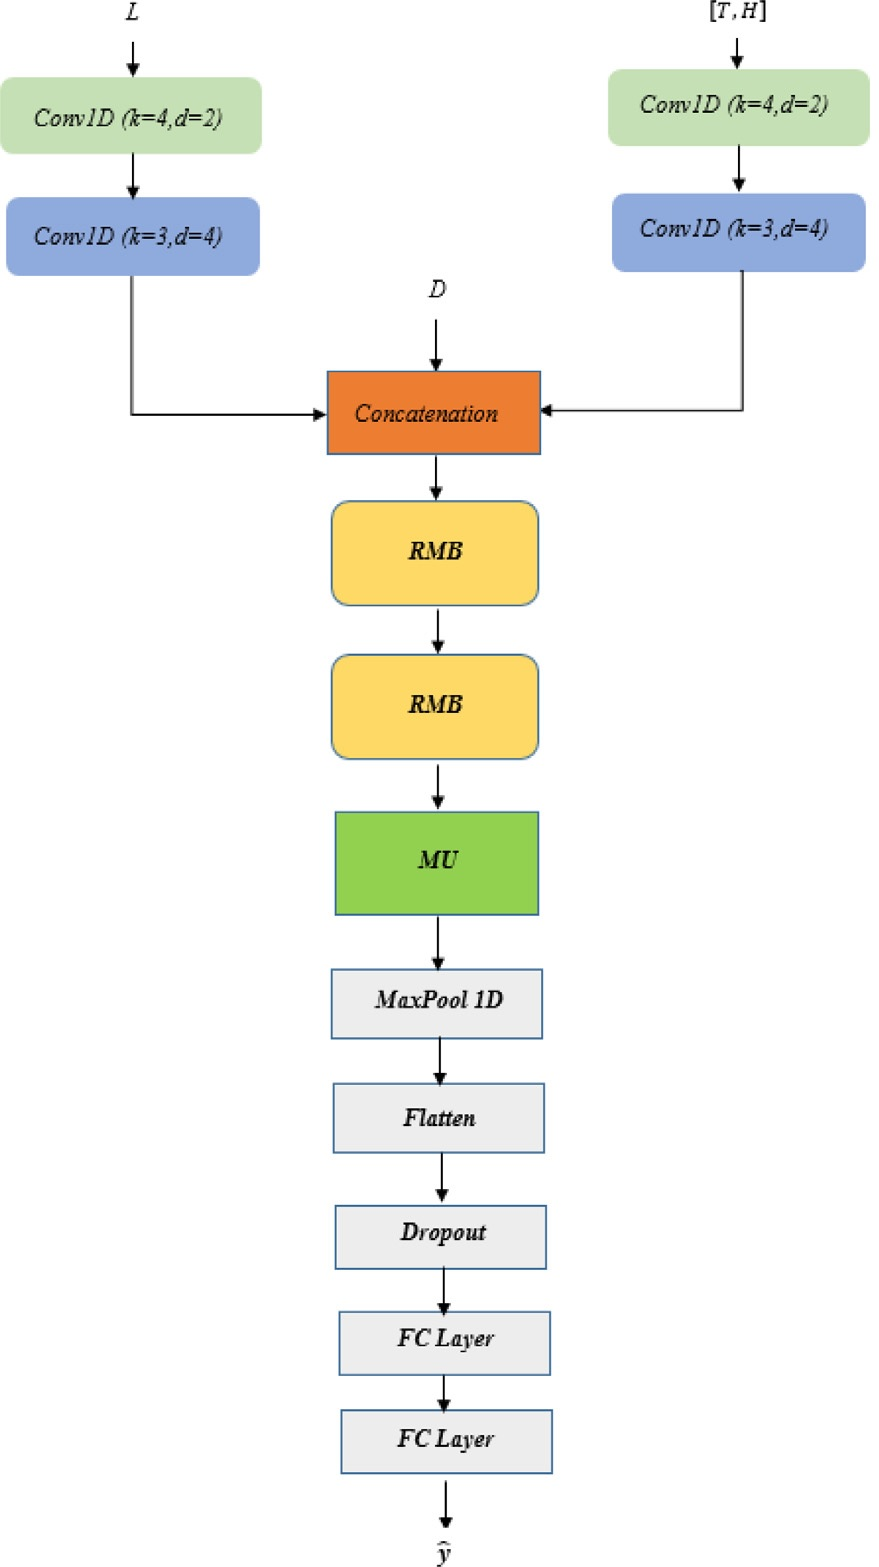
\includegraphics[width=0.5\columnwidth]{Final Report/Figures/Yazici2022_1DCNN.jpg}}
\caption{The 1D-CNN model architecture proposed by \cite{Yazici2022}.}
\label{1DCNN}
\end{figure}

This network utilises Residual Multiplicative Blocks (RMBs; see Figure \ref{RMB}), an essential ingredient in VPNs, and a Multiplicative Unit (MB; see Figure \ref{MU}), initially used for video processing problems. The MU used in \cite{Yazici2022} comprises gates merged into a convolutional layer and implements some slight modifications to the original method used by \cite{Kalchbrenner2017}, resulting in performance improvements.

\begin{figure}[H]
    \centering
    \includegraphics[width=1.0\linewidth]{Final Report//Figures/Yazici2022_RMB.png}
    \caption{The RMB module structure used in \cite{Yazici2022}.}
    \label{RMB}
\end{figure}

\begin{figure}[H]
    \centering
    \includegraphics[width=0.8\linewidth]{Final Report//Figures/Yazici2022_MU.png}
    \caption{The MU structure used by \cite{Yazici2022}.}
    \label{MU}
\end{figure}

\section{Performance Measures}
The mean squared percentage error (MAPE) is commonly used for time series predictions, often with the addition of a regularisation penalty \cite{Gasparin2021}. The calculation is provided in Equation \ref{f-MAPE}, where $L_A$ is the actual load, $L_F$ is the forecast load, $N$ is the number of hours, and $i$ is the time step index.

\begin{equation}\label{f-MAPE}
    MAPE = \frac{100}{N} \sum^{N}_{i=1} {\frac{\left|L_A^i - L_F^i\right|}{L_A^i}}
\end{equation}

Authors in \cite{Hippert2001} argued that while the MAPE has become the industry standard, it is not enough to assess model performance and that the loss function associated with the forecasting errors should be used in model evaluation, as is detailed extensively in \cite{Smith2018}.



\bigskip

\hypertarget{material-and-methods}{%
\chapter{Material and Methods}\label{material-and-methods}}

\hypertarget{software}{%
\section{Software}\label{software}}
In the execution of this project, various software tools were utilised to perform analyses, manage data, and facilitate the computational aspects. The primary tools we used were as follows.

\textbf{\textit{Python}.} \textit{Python} served as the primary tool for data analysis in this project, chosen for its comprehensive selection of machine learning packages and accessible entry level. Additionally, given the project's emphasis on constructing neural networks to forecast demand, the \textit{TensorFlow} framework was employed, offering robust support for \textit{Python}. Other \textit{Python} packages used included \textit{Matplotlib} and \textit{seaborn} for visualisations, \textit{Schemdraw} for diagrams, \textit{Pandas} for managing tables, and \textit{NumPy} and \textit{SciPy} for statistical operations.

\textbf{\textit{MongoDB}.} \textit{MongoDB} was utilised as the core database to maintain one central data source throughout data analysis and model building. As a scalable, cloud-hosted No-SQL database, \textit{MongoDB} adeptly manages the project's substantial data volume. Its No-SQL architecture supports a wide range of data structures, proving particularly effective for storing tensors.

\textbf{\textit{Bash}.} \textit{Bash} was employed for the initial loading of raw data into \textit{MongoDB}. It was chosen for its minimal overhead and compatibility across all operating systems.

\textbf{\textit{Git}.} \textit{Git} was used to manage and synchronise changes across team members, including \textit{Python} code and \textit{Markdown} meeting agendas and minutes. This version control system is essential for coordinating team efforts, allowing for seamless collaboration, historical tracking of project changes, and the ability to revert to previous versions if necessary, ensuring consistency and accuracy in the development process.

\textbf{\textit{GitHub}.} \textit{GitHub} was used to remotely host the repository for the project, providing redundancy against code loss or corruption. This platform not only ensures secure storage of all project artifacts but also facilitates easy access and collaboration among team members, regardless of their location, enhancing the robustness and reliability of the development process.

\textbf{\textit{Overleaf}.} All reports were written in \LaTeX and coordinated through \textit{Overleaf}. \LaTeX is a powerful markup language that enables professional reports to be easily produced. It also integrates well with Python, as \textit{Pandas} tables can be saved as TEX files and read directly into reports. \textit{Overleaf} extends these capabilities to collaborative efforts, allowing the team to write and review our documents simultaneously.

\hypertarget{description-of-the-data}{%
\section{Description of the Data}\label{description-of-the-data}}
This section provides a detailed overview of the data utilised in the project, including the storage of data in \textit{MongoDB}, comprehensive data dictionaries, and high-level statistical summaries of the data sets, such as file sizes and quantities. \newline

This project will use two input data sources that provide total demand (TD) data and temperature (Temp) data for several Australian states spanning 2010 to 2021. Summary statistics for the two datasets can be found in the table below.

\CatchFileDef{\metadata}{"Final Report/Tables/source-file-statistics.tex"}{} \metadata

These source datasets were stored as separate collections in a \textit{MongoDB} database. High-level data dictionaries, including field definitions and field statistics, have been included below.

\begin{landscape}

    \CatchFileDef{\tdemand-dict}{"Final Report/Tables/total-demand-data-dictionary-formatted.tex"}{} \tdemand-dict

    \CatchFileDef{\temp-dict}{"Final Report/Tables/temperature-data-dictionary-formatted.tex"}{} \temp-dict
    
\end{landscape}

\hypertarget{pre-processing-steps}{%
\section{Pre-processing Steps}\label{pre-processing-steps}}

A data pre-processing pipeline was used to clean, aggregate, enrich, and transform raw data sources stored in \textit{MongoDB} into a collection of features used by the neural network models. The key steps were as follows (see Appendix \ref{appendix-preprocessing-pipeline} for the process flow diagram for this pipeline).

\textbf{Read Data.} We ingested the total\_demand and temperature datasets from \textit{MongoDB} collections and converted them to \textit{dataframes}.

\textbf{Merge Datasets.} We joined the temperature data with the demand data to create a consolidated feature set. This step also included removing the location information from the temperature source, as it was not used for building the models.

\textbf{Impute missing values.} We used an iterative imputation method to fill any missing values. This imputation is particularly important, as missing values may be introduced into the temperature readings due to the merge.

\textbf{Split Datetime.} We separated the timestamps into their components for modelling. These components included the year, month, and day of the week.

\textbf{Calculate Daylight.} We enriched the data using the \textit{astral} \textit{Python} package and calculated whether a record was taken during daylight.

\textbf{Calculate Public Holiday.} We enriched the data using the \textit{holidays} \textit{Python} package and calculated whether a record was taken during a public holiday.

\textbf{Transform periodic features:} We performed a polar transformation on periodic features (e.g., the month, day of the week).

\textbf{Combine Features.} We consolidated all engineered features into a single dataset.

\textbf{Dependent Variables Added.} We added the total demand data for 1 and 24 hours into the future to be used as the predicted variables when training the neural network for short-term forward prediction of the total\_demand.

\textbf{Write Features.} We wrote the processed and cleaned feature dataset to a collection in \textit{MongoDB}.

\hypertarget{read-data}{%
\subsection{Read Data}\label{pre-processing-steps}}
To leverage \textit{Python}'s extensive data processing capabilities and robust package support, the data was extracted from \textit{MongoDB} using the \textit{pymongo} API and converted into a \textit{DataFrame} for manipulation.

\hypertarget{merge-datasets}{%
\subsection{Merge Datasets}\label{merge-datasets}}
The local temperature is a key variable when predicting the total demand, necessitating the merging of temperature and demand datasets. The location field was also removed from the temperature dataset, as it is not necessary for demand prediction in its current form \cite{DeCian2007}.

\hypertarget{impute-missing}{%
\subsection{Impute Missing Values}\label{impute-missing}}
To build an effective model, the dataset must first be cleaned. This process includes imputing missing values. In this investigation, iterative imputation is employed, which utilises regression techniques to estimate missing values based on the relationships with other variables in the dataset, thereby preserving the kurtosis of the data. Maintaining the kurtosis is crucial as it ensures that the tail-heaviness or the peakedness of the distribution remains consistent, which is vital for the accuracy of statistical models and the validity of inferred conclusions \cite{Hoque2021}.

\hypertarget{split-datetime}{%
\subsection{Splitting Timestamp Feature}\label{split-datetime}}
In the pre-processing pipeline, the date-time feature was split into its components to enhance the accuracy of the machine learning models, providing detailed temporal insights that allowed for more precise capture of seasonal and cyclic trends. These components include the year, month, day of the month, day of the week, whether it is a weekday, and the period of day\footnote{This corresponds to splitting a single day into 48 periods to represent the data at its 30-minute granularity.}.

\hypertarget{calculate-daylight}{%
\subsection{Calculating Daylight}\label{calculate-daylight}}
To further enrich the feature set, the timestamps were utilised with the \textit{astral} package to determine whether a given record was taken during daylight hours. Daylight is a key factor in predicting demand, as daylight typically corresponds with reduced power usage in homes due to people being at work. Please note that this calculation incorporated the 'state' field to account for variations in daylight hours by location.

\hypertarget{calculate-public-holiday}{%
\subsection{Calculating Public Holidays}\label{calculate-public-holiday}}
Similarly, the \textit{holidays} package was used to determine whether a timestamp fell on a public holiday. This was also a key feature in helping to account for spikes in demand caused by community events or increased home power usage on public holidays. This calculation also incorporated the 'state' field since the public holiday schedule differs by state.

\hypertarget{transform-periodic}{%
\subsection{Transforming Periodic Features}\label{transform-periodic}}
The pre-processing pipeline employed a polar coordinate transformation to encode periodic date-time features, ensuring that models effectively capture the cyclical and seasonal patterns. As described in Section \ref{Pre-Processing and Feature Engineering}, this method enhances adjacency and periodicity, which is crucial for accurate and efficient model training. The logic for this transformation is described below.

\hypertarget{write-features}{%
\subsection{Writing Feature Set to \textnormal{MongoDB}}\label{write-features}}
Finally, after applying all transformations and cleaning operations, the processed features were stored in \textit{MongoDB}, ready for integration into the modelling process. This was also performed using the \textit{MongoDB} API.

\hypertarget{ohe}{%
\subsection{One-Hot Encoding}\label{ohe}}

As our \textit{MongoDB} cluster had limited storage, the final pre-processing stage was performed locally with \textit{Python}. This firstly involved one-hot encoding of the state variable using \textit{scikit-learn}. The original string column of state names was then removed.

\hypertarget{univariate-gen}{%
\subsection{Generate Univariate Inputs}\label{univariate-gen}}

The second local process was generating the univariate columns. For this, a loop was used to join the table 48 times with an offset copy of itself in which the timestamp was increased in 30-minute intervals. These joins added 48 new variables to the dataset that showed the total demand for the past 24 hours, inclusive. As this created empty values in the newest and oldest records in the dataset, all records with a null value were removed from the table. The univariate approach was adopted because demand exhibits continuity over short intervals, making its immediate history a strong predictor of near-future conditions. By utilising these specific time lags, the model can effectively capture daily and hourly fluctuations, which is crucial for accurate forecasting in scenarios where routine human activities and natural cycles heavily influence demand patterns.

\hypertarget{data-scaling}{%
\subsection{Data Scaling}\label{data-scaling}}

The final transformation of the data before training the models was standardising each variable using Function \ref{f-scale}, where $x$ is a single value, $\mu$ is the variable's mean, and $s$ is the variable's standard deviation. This transformation centres the variable's distribution around zero and changes the individual values to their standard deviations from the mean without changing the shape of the data. By placing all variables on the same scale, this standardisation stops any variable from dominating the model by having a larger magnitude.

\begin{align}\label{f-scale}
f_{\text{scale}}(x) &= \frac{x-\mu}s
\end{align}

\hypertarget{train-val-test}{%
\subsection{Train, Validation, and Test Splitting}\label{train-val-test}}

The data were split into train, validation, and test sets to develop and test the models. As the data are for time-series modelling, they were sorted chronologically before splitting. The most recent 20 per cent of the data were reserved for testing. To ensure the validity of the process, these data remained "unseen" by the models or modeller until the final tests. The older 80 per cent of the data were then split five times into training and validation sets for time-series cross-validation. For this process, the oldest $\frac16$ of the data are used to forecast the second oldest $\frac16$. Then the oldest $\frac1{3}$ are used to forecast the third oldest $\frac16$. This pattern repeats until the oldest $\frac56$ of the data are used to forecast the most recent $\frac16$. The mean validation MAPE of these rolling forecast origins is then used to determine which model variant performs best \cite{hyndman2018}. The train-validation data were used for model development and hyperparameter tuning. After this, the models were retrained on the entire train set (i.e. 80\% of the data) and validated on the test set. The results reported below were subsequently generated from the test set.

\hypertarget{features-reduction}{%
\subsection{Feature Reduction}\label{features-reduction}}

After engineering various features and consolidating the training data, an attempt was made with L1 regularisation to reduce the number of features used in the final models. This reduction would benefit the models by decreasing training time and reducing the data required to utilise them. The subsequent results are outlined in Table \ref{feat-red}. A deep multivariate MLP with L1 regularisation factor $\lambda_{L1}=0.1$ on the kernel weights was trained on the NSW data for 2000 epochs. The subsequent model was used to exclude the least impactful variables from the model. The kernel weights relating to each variable throughout the neural network were summed, and variables with sums falling below $\epsilon$ were excluded. The $\epsilon$ values $10^{-3}$ and $10^{-4}$ were reviewed. The results showed that removing low-impact variables was preferable to simply using L1 regularisation, as it decreased training time and improved the MAPE. However, the acceleration was only modest, and the validation loss deteriorated, compared to the unregularised model, more than mild improvements in training time could justify. As such, all features were included in the final model tests.

\CatchFileDef{\feat-red}{Tables/feature reduction.tex}{} \feat-red

\hypertarget{assumptions}{%
\section{Assumptions}\label{assumptions}}
When conducting feature engineering, three key assumptions were made to obtain a valid set of features. The first assumption is that the temperature data from a specific location within the city was applied to the entire state. This assumption is considered valid because a significant portion of the demand originates from the city. The second is that daylight calculations were based on the capital city's data. However, it is recognised that temperature variations can be substantial across different areas of the state. The third is that the identification of public holidays was based on the schedule of the capital city, despite known variations in holiday observance across different regions. 

Assumptions were also made during the modelling. Given the size of the dataset, model architecture experimentation, including hyperparameter grid-search cross-validation, utilised only the data from NSW. This step dramatically accelerated experimentation, which was necessary given the time constraints of the project. However, it meant that the process assumed that the patterns within the NSW data would apply to all states. There are good reasons, such as environmental and economic differences, to doubt this assumption, but it was necessary given the current limitations. Similarly, the grid search for the hyperparameters was only performed on the shallow multivariate versions of the MLP and BD-LSTM. The generalisability of these results is unclear, but we needed to assume this would be sufficient due to the considerable time constraints. For the same reason, we also assumed that Adam optimisation would be optimal and conducted our tests accordingly. This assumption, of course, violates the "no free lunch" theorem. The final assumption made during modelling is that issues of model complexity and comprehensibility would be irrelevant to our report. These factors are often considered important. However, as we only review neural networks, which are always somewhat complex and never readily comprehensible, we deemed this consideration superfluous to our modelling. Subsequently, only runtime performance, goodness of fit, and forecast accuracy were considered.

\hypertarget{modelling-methods}{%
\section{Modelling Methods}\label{modelling-methods}}

\hypertarget{model-design}{%
\subsection{Model Design}\label{model-design}}

Two broad models were used in this report: multilayer perceptrons (MLPs) and bidirectional long short-term models (BD-LSTMs).\footnote{The team also hoped to include a one-directional convolutional neural network, but time and technical constraints ultimately made this infeasible.} Four variants were created for both of these models: univariate, multivariate, deep, and shallow, with eight models ultimately being instantiated and tested. The univariate models took 49 inputs. These covered the total demand values from the time of the record to 24 hours beforehand, inclusive, in half-hour intervals. The multivariate models, taking 70 inputs, included these 49 inputs, temperature, and various engineered features (see Section \ref{pre-processing-steps}). The univariate models both had one hidden layer.\footnote{The BD-LSTM technically had two hidden layers, as the bidirectional layer consists of two layers: one parsing the data forward and the other backward.} The deep MLPs had ten hidden layers, whereas the deep BD-LSTMs had two bidirectional layers. With one exception, all hidden layers had 32 units. The deep BD-LSTM had 64 units in its first layer, making this model both wider and deeper. All BD-LSTM hidden layers used a tanh activation function. The shallow MLPs used relu in its hidden layer, and the deep MLP alternated between relu and linear. All output layers used a linear activation function and produced two outputs covering the one-hour-ahead and 24-hour-ahead prediction horizons.

\begin{figure}[H]
\centerline{\includegraphics[width=\columnwidth]{Figures/Diagrams/BD-LSTM deep.pdf}}
\caption{The architecture of the uni- and multivariate deep BD-LSTMs. The deep variants have two hidden bidirectional LSTM units. The univariate model takes 49 inputs and delivers two outputs, and the multivariate model takes 70 inputs and delivers two outputs. Each bidirectional unit has two layers: one parsing the data forward and the other backward. Both directional layers take inputs from the layer before the bidirectional unit and pass their outputs to the layer following the bidirectional unit. All hidden layers use a tanh activation function. The output uses a linear or identity activation.}
\label{lstm_deep}
\end{figure}

\begin{figure}[H]
\centerline{\includegraphics[width=0.9\columnwidth]{Figures/Diagrams/MLP deep.pdf}}
\caption{The architecture of the uni- and multivariate deep MLPs. The deep variants have ten hidden layers. The univariate model takes 49 inputs and delivers two outputs, and the multivariate model takes 70 inputs and delivers two outputs. The hidden layers alternate between relu and linear or identity activation functions. The output uses a linear or identity activation.}
\label{mlp_deep}
\end{figure}

\begin{figure}[H]
\centerline{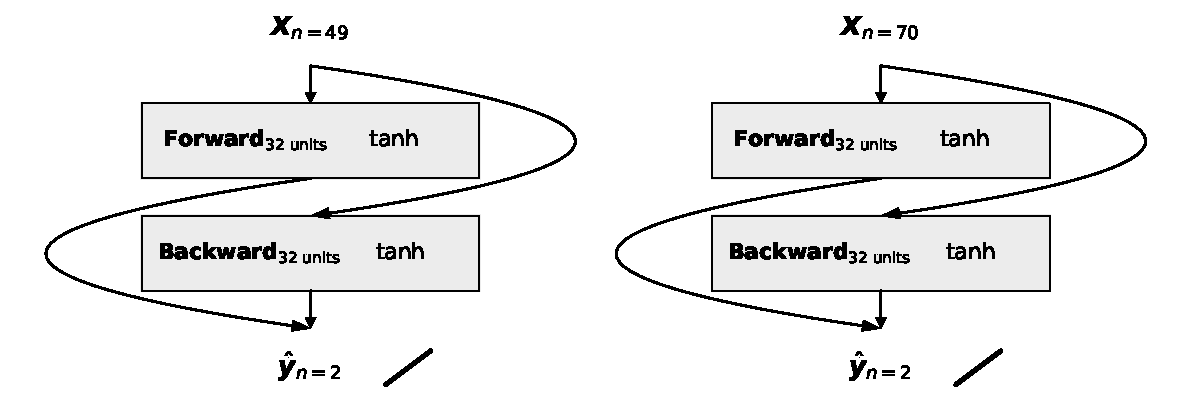
\includegraphics[width=\columnwidth]{Figures/Diagrams/BD-LSTM Shallow.pdf}}
\caption{The architecture of the uni- and multivariate shallow BD-LSTMs. The shallow variants have one hidden bidirectional LSTM unit. The univariate model takes 49 inputs and delivers two outputs, and the multivariate model takes 70 inputs and delivers two outputs. The bidirectional unit has two layers: one parsing the data forward and the other backward. Both directional layers take inputs from the input layer and pass their outputs directly to the output layer. Both hidden layers use a tanh activation function. The output uses a linear or identity activation.}
\label{lstm_shallow}
\end{figure}

\begin{figure}[H]
\centerline{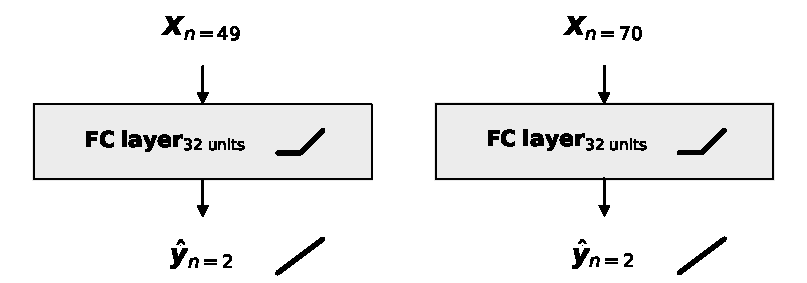
\includegraphics[width=.7\columnwidth]{Figures/Diagrams/MLP Shallow.pdf}}
\caption{The architecture of the uni- and multivariate shallow MLPs. The deep variants have one hidden layer. The univariate model takes 49 inputs and delivers two outputs, and the multivariate model takes 70 inputs and delivers two outputs. The hidden layer has a relu activation functions. The output uses a linear or identity activation.}
\label{mlp_shallow}
\end{figure}

\hypertarget{hyperparam-tuning}{%
\subsection{Hyperparameter Tuning}\label{hyperparam-tuning}}

Given the project's time constraints, we used larger batch sizes and learning rate scheduling that included a large learning rate to accelerate training \cite{Smith2018}. Beyond acceleration, larger batch sizes and learning rates contribute to model regularisation, making these adjustments broadly beneficial. For the batch size, we tested models using $2^8$, $2^9$, and $2^{10}$ (see Table \ref{param-grid}). The learning rate was scheduled to adjust between epochs (i.e. the step size was set at one epoch), alternating between a large and a small rate. To find an appropriate learning rate schedule, an experiment was run using five-fold cross-validation to compare these four scheduling functions, where the function's output provides the learning rate for the current epoch. 
\begin{align}
f_1 &=  \text{IF } \text{epoch} \% 2 = 1 \text{ THEN }10^{-4} \text{ ELSE }10^{-3} \\
f_2 &=  \text{IF } \text{epoch} \% 2 = 1 \text{ OR } \text{epoch}>\frac{\text{epoch}}2 
        \text{ THEN }10^{-4} \text{ ELSE }10^{-3} \\
f_3 &=  10^{-4} \\
f_4 &=  \text{IF } \text{epoch} \% 2 = 1 \text{ OR } \text{epoch}>\text{epoch}-100
        \text{ THEN }10^{-4} \text{ ELSE }10^{-3}
\end{align}
The first function alternates the learning rate at every epoch. The second alternates for only the first half of all epochs before only using the lower rate. The third only uses the lower rate. The fourth alternates until the last 100 epochs, for which it only uses the lower rate. The results, shown in Figure \ref{lr_sched}, indicate that $f_4$ performs best. However, when reviewing the training histories (see Figure \ref{lr_hist}), we can see that, beginning around epoch 1900, the training curve for $f_4$ improves significantly while its validation curve deteriorates. This divergence indicates overfitting \cite{Ng2018}. Fortunately, $f_1$ performed similarly well and showed no signs of misspecification. As such, $f_1$ was used in all subsequent modelling.

\begin{figure}[H]
\centerline{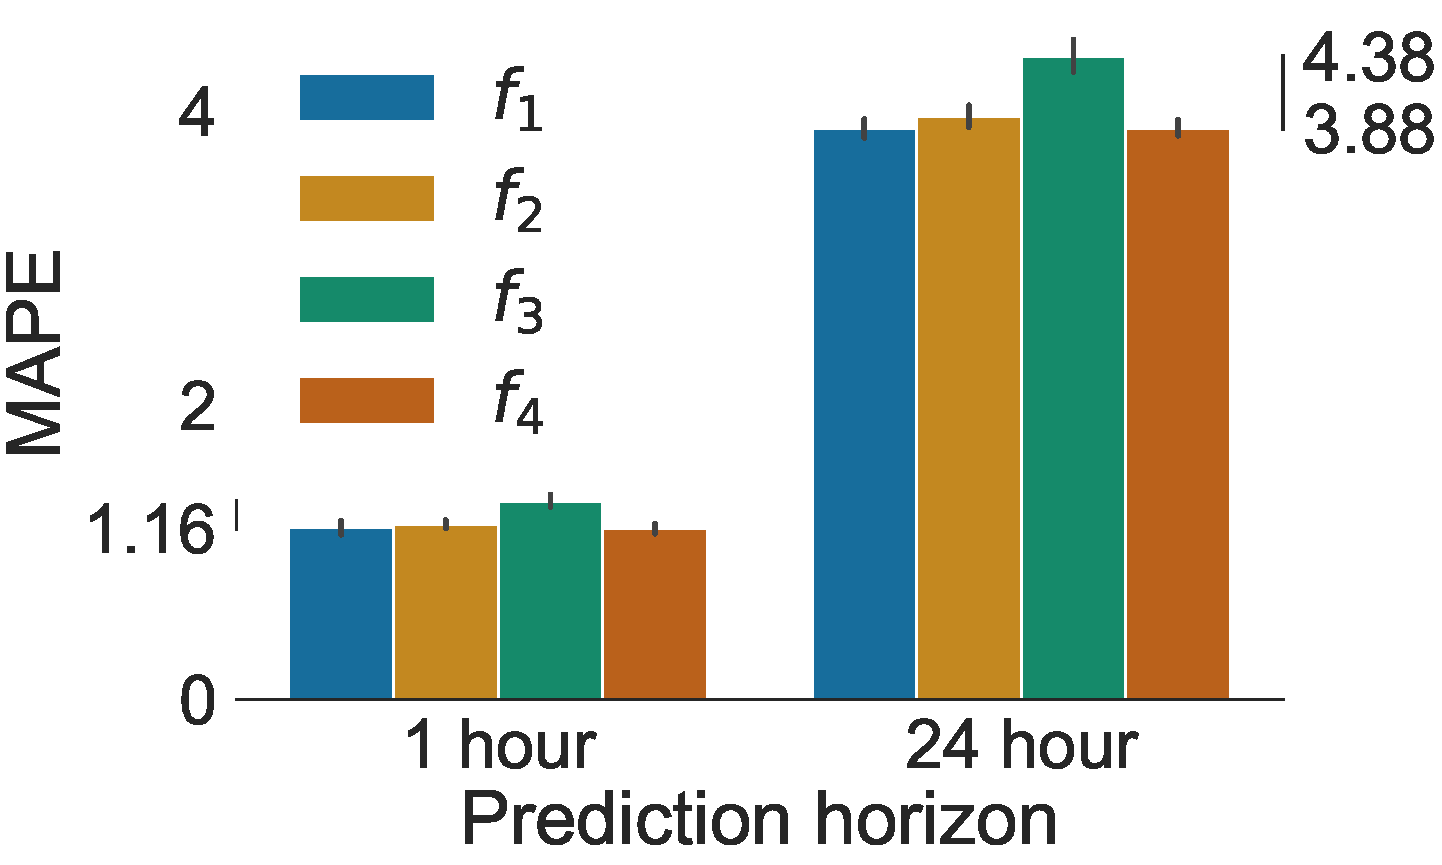
\includegraphics[width=.6\columnwidth]{Figures/Plots/LR scheduling experiment results.pdf}}
\caption{Results of the learning rate scheduling experiment showing the MAPE (CI: 95\%) for both prediction horizons for each function.}
\label{lr_sched}
\end{figure}

\begin{figure}[H]
\centerline{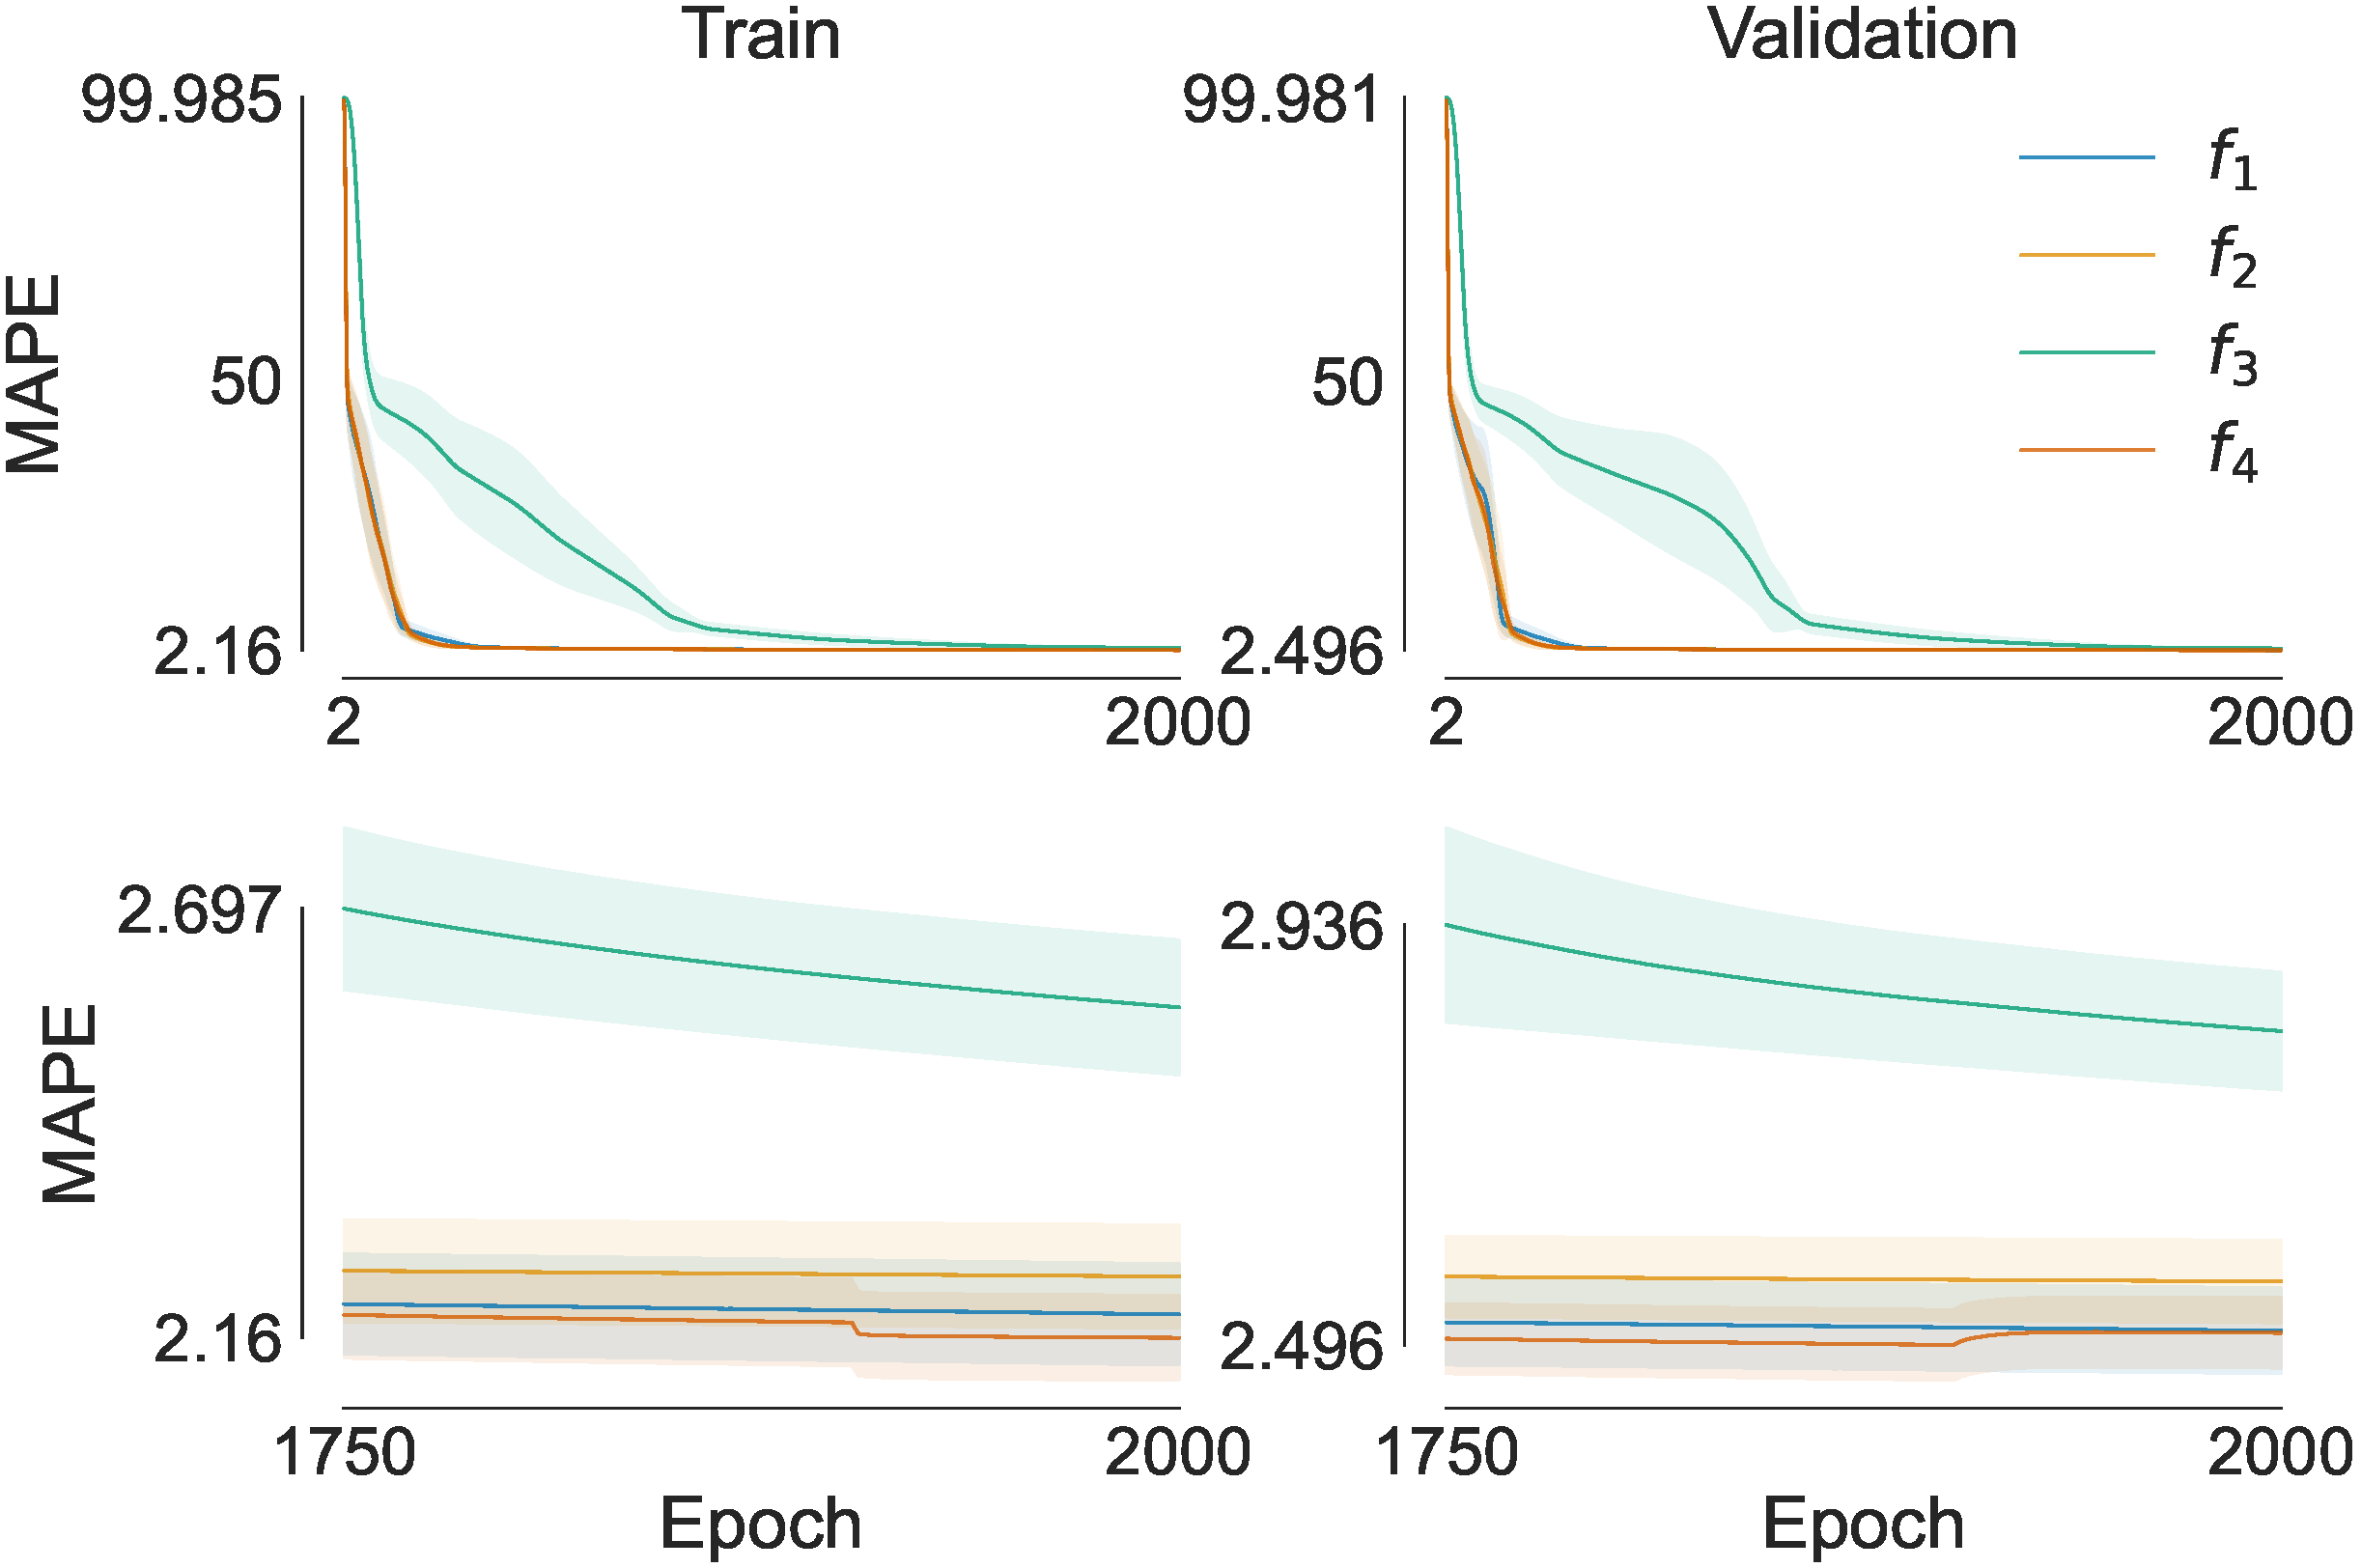
\includegraphics[width=\columnwidth]{Figures/Plots/LR scheduling experiment training histories.pdf}}
\caption{Training histories from the learning rate scheduling experiment showing the test and validation MAPE (CI: 95\%). Due to their significance, the final 250 epochs are shown in greater detail.}
\label{lr_hist}
\end{figure}

For the remaining hyperparameter tuning, a grid search with five-fold cross-validation was used to select the optimal hyperparameters. A shallow multivariate version of both models was used to estimate the optimal hyperparameter combination for each group of models. A parameter grid (Table \ref{param-grid}) covering 27 combinations of batch size, weight decay, and momentum ($\beta_1$) was searched. The combination resulting in the best mean results from the cross-validation was selected. For both MLPs and BD-LSTMs, a batch size of $2^8$ and weight decay of $10^{-5}$ were optimal. The MLP performed better with a momentum of 0.95, whereas the BD-LSTM performed better with $\beta_1=0.8$.

\CatchFileDef{\param-grid}{Tables/parameter grid.tex}{} \param-grid
\CatchFileDef{\gsearch-res}{Tables/grid search results.tex}{} \gsearch-res

\hypertarget{model-training}{%
\subsection{Model Training}\label{model-training}}

To train the models before producing the final results, we initially ran each model for approximately two hours. As BD-LSTMs train on the data recurrently, they take magnitudes longer to complete the same number of epochs as an MLP (see Table \ref{ttimes}). For instance, the univariate shallow MLP completed 10,500 epochs in slightly under two hours. In a comparable amount of time, the univariate shallow BD-LSTM completed 105 epochs. The slowest model was the multivariate deep BD-LSTM, which only completed 21 epochs within two hours. Once this first round of training was completed, the learning curves were analysed, and it was determined that the MLPs were sufficiently trained. The remaining training was then shared between the team to accelerate the process. Unfortunately, however, we ultimately lacked sufficient time to train the models to optimality (see Section \ref{learning-curve-analysis}). Total training times and epochs are listed in Table \ref{tsummary}.

\CatchFileDef{\ttimes}{Tables/train times.tex}{} \ttimes
\CatchFileDef{\tsummary}{Tables/training summary.tex}{} \tsummary

\hypertarget{exploratory-data-analysis}{%
\chapter{Exploratory Data Analysis}\label{exploratory-data-analysis}}
The exploratory data analysis focused on identifying key features significantly impacting the total demand. Visual analysis and correlation assessments were performed to determine key predictors for inclusion in the machine learning models. This process was critical in enhancing the accuracy and efficiency of the predictive outcomes.

\hypertarget{demand-distributions}{%
\section{Total Demand Distributions}\label{demand-distributions}}

\begin{figure}[H]
\centerline{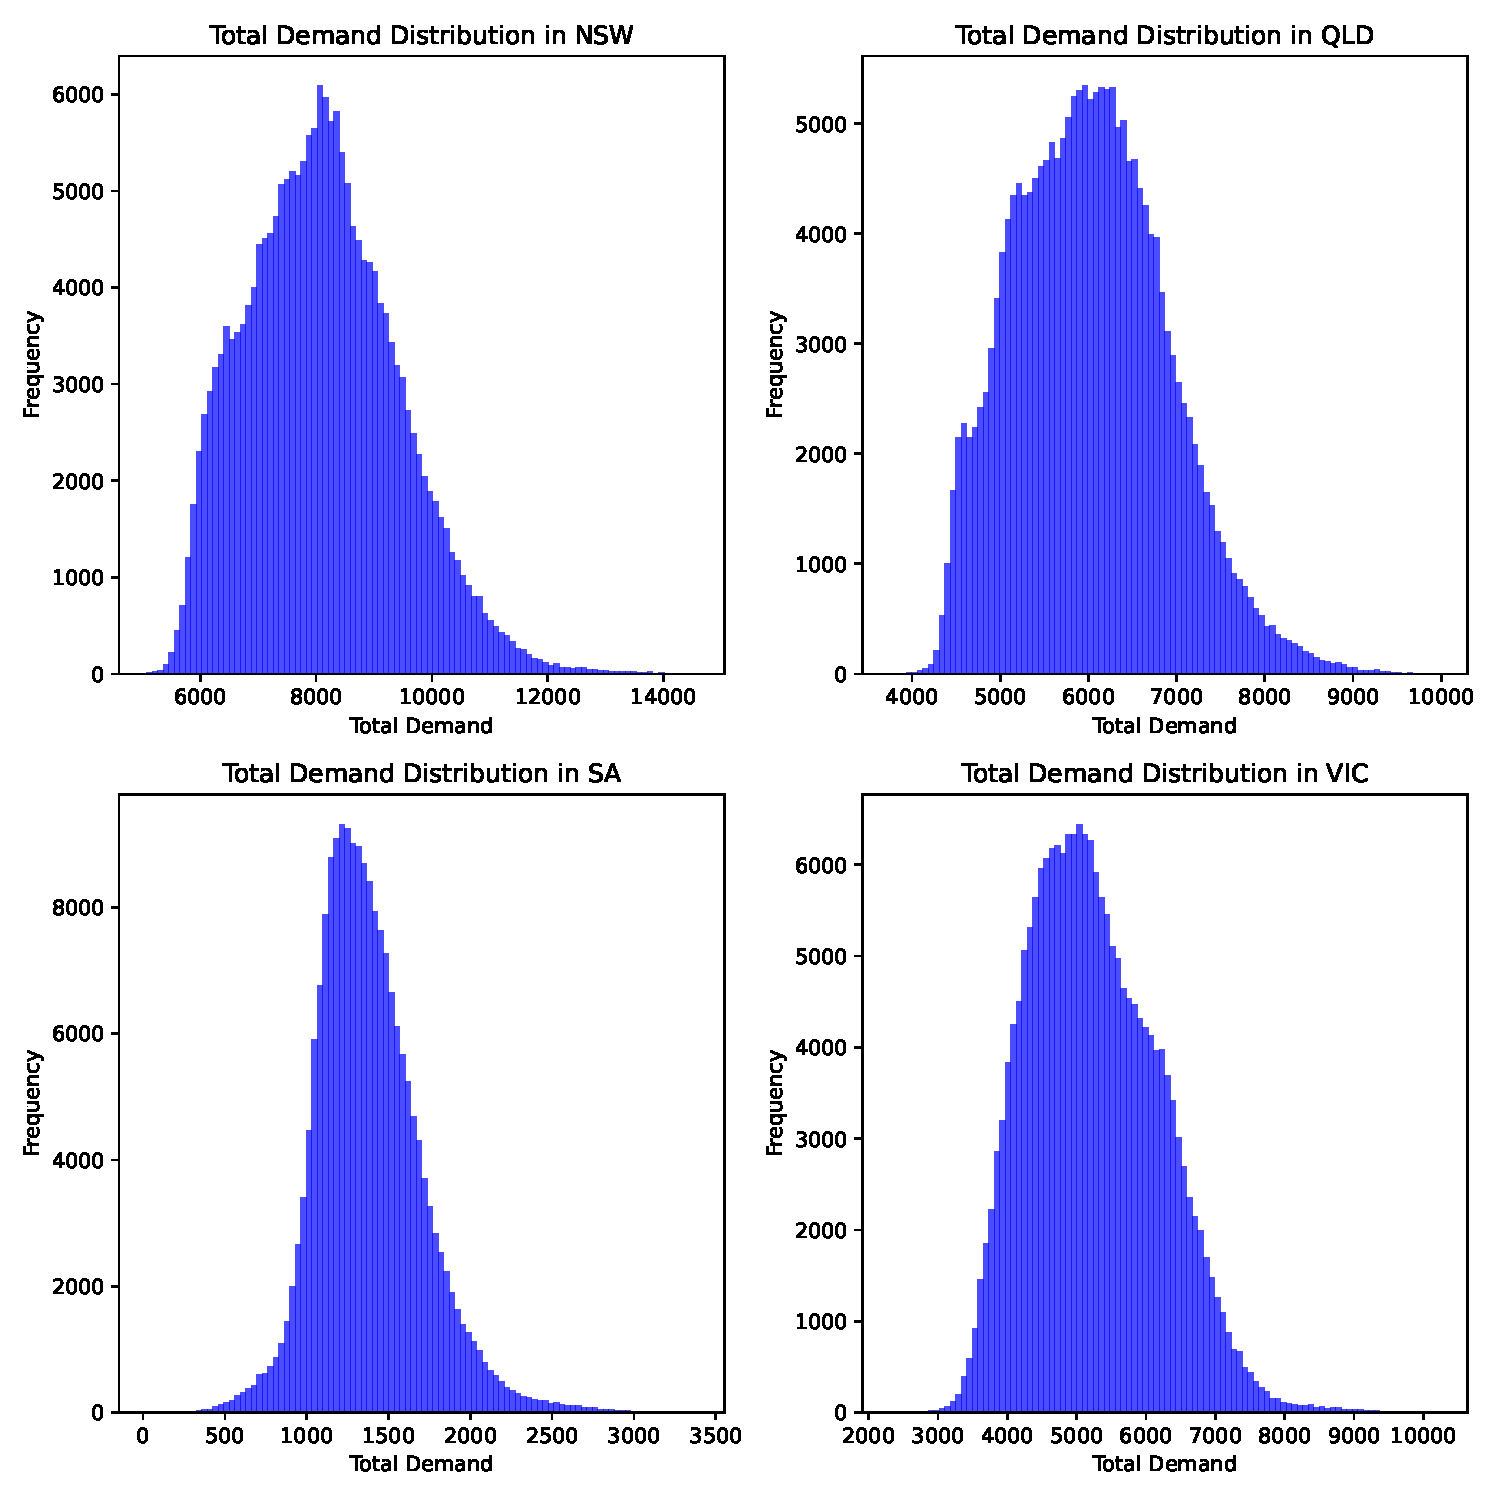
\includegraphics[width=\columnwidth]{Final Report/Figures/Plots/total_demand_distribution.pdf}}
\caption{Histograms of total demand for NSW, QLD, SA and VIC}
\label{demand-distributions-plot}
\end{figure}
Figure \ref{demand-distributions-plot} shows that each state's demand data is approximately normal. This stability helped facilitate faster and more stable convergence during training since the activation functions typically perform better with inputs that avoid extreme values. Each distribution displays a leptokurtic shape with some right skew, indicating that demand typically concentrates around the mean with some high-demand outliers.

\hypertarget{temperature-distributions}{%
\section{Temperature Distributions}\label{temperature-distributions}}

\begin{figure}[H]
\centerline{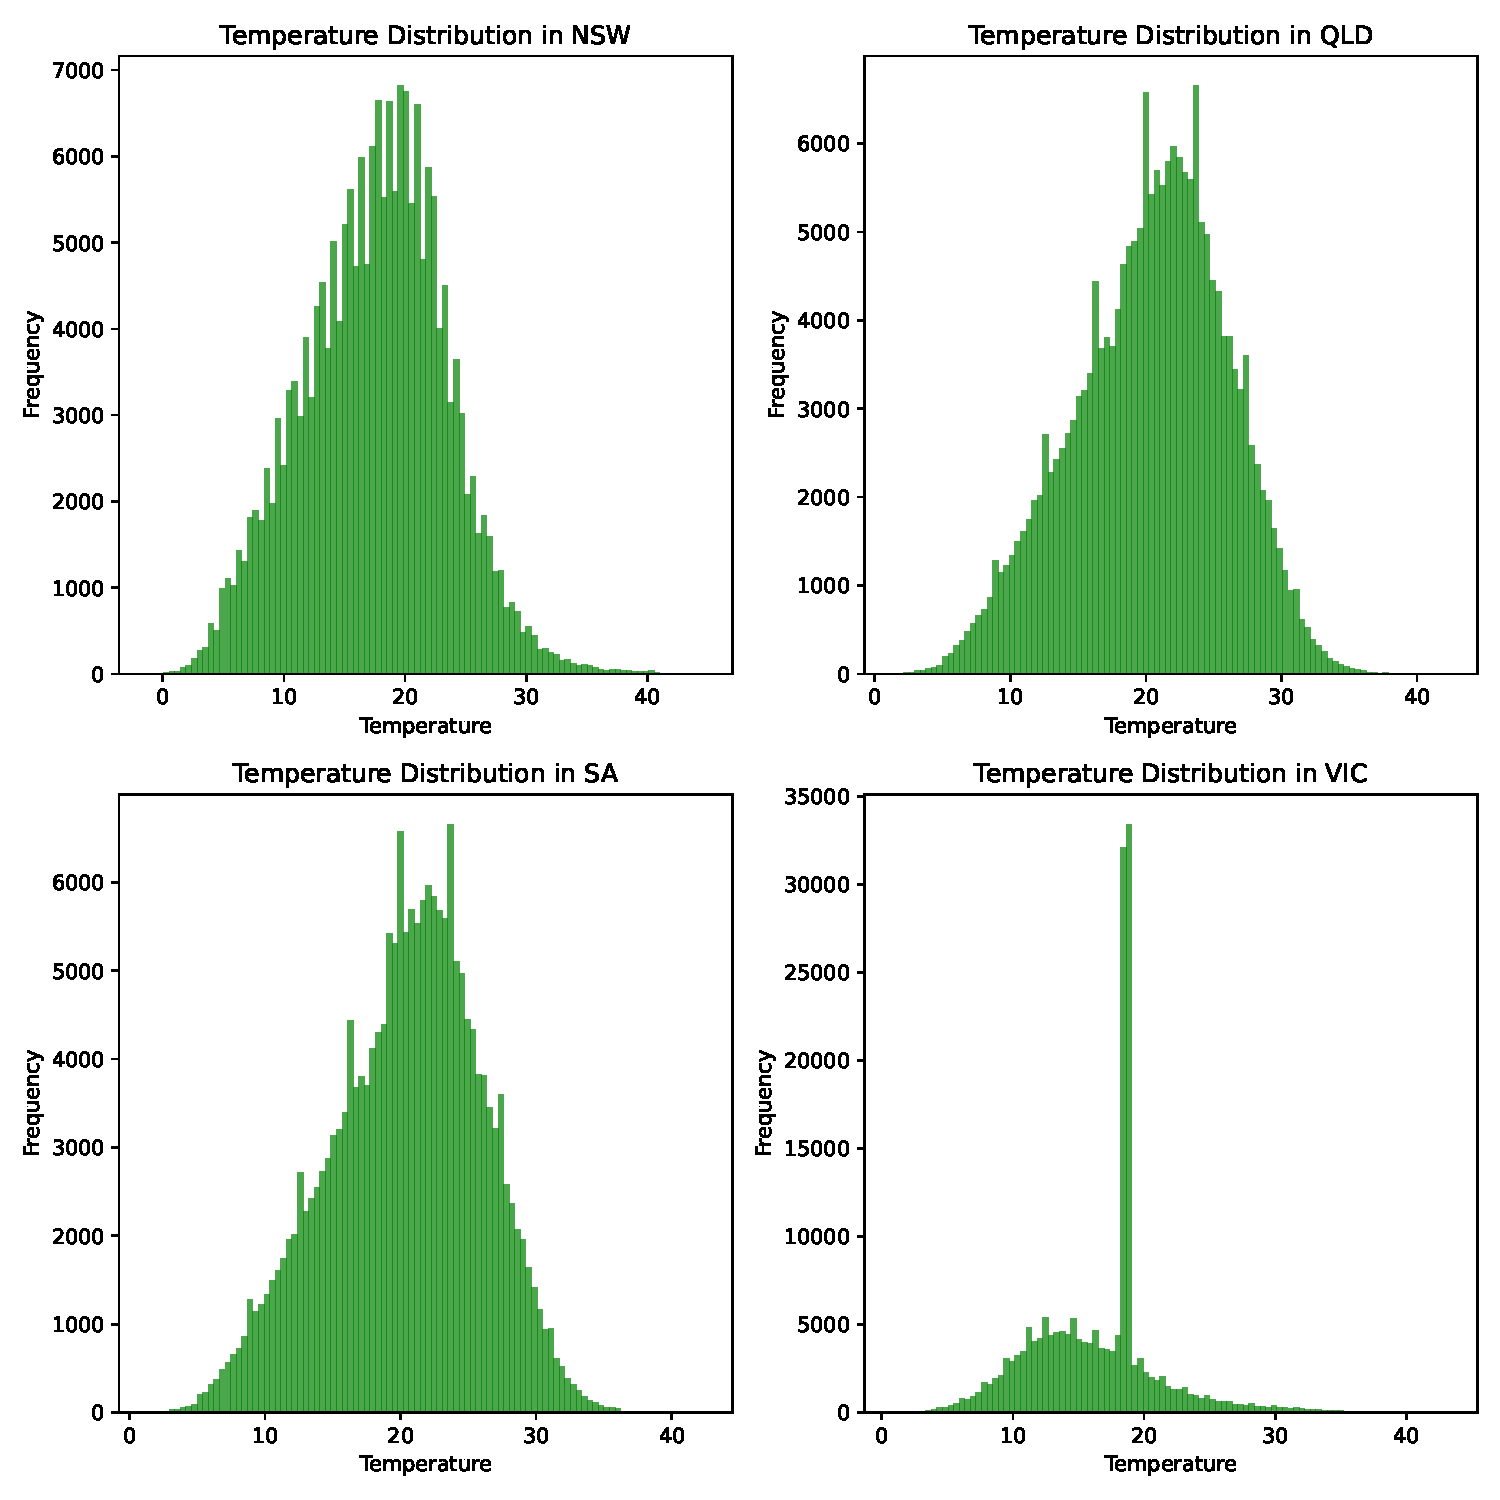
\includegraphics[width=\columnwidth]{Final Report/Figures/Plots/temperature_distribution.pdf}}
\caption{Histograms of temperature for NSW, QLD, SA and VIC}
\label{temperature-distributions-plot}
\end{figure}

The temperature distributions in Figure \ref{temperature-distributions-plot} follow a similar leptokurtic approximately normal distribution. The distributions also exhibit several peaks that can be attributed to the lesser granularity of the temperature data, resulting in common values occurring more frequently. In the VIC dataset, a substantial peak occurs around the mean. This peak resulted from imputing the missing values that entered the dataset when merging with the temperature and total demand data.

\hypertarget{correlation-scatter}{%
\section{Correlation Scatter}\label{correlation-scatter}}

\begin{figure}[H]
\centerline{\includegraphics[width=\columnwidth]{Final Report/Figures/Plots/demand_vs_temperature_scatter.png}}
\caption{Demand vs. Temperature Correlation}
\label{correlation-scatter-plot}
\end{figure}

The scatter plots in Figure \ref{correlation-scatter-plot} show a strong quadratic correlation between temperature and demand. This correlation can be attributed to increased heating or cooling for extreme temperatures. Interestingly, the quadratic relationship for SA is negative. However, by inspecting the plot, we can see that a higher-order function may better represent the relationship.

\hypertarget{periodic-box-plots}{%
\section{Periodic Feature Box Plots}\label{periodic-box-plots}}

\begin{figure}[H]
\centerline{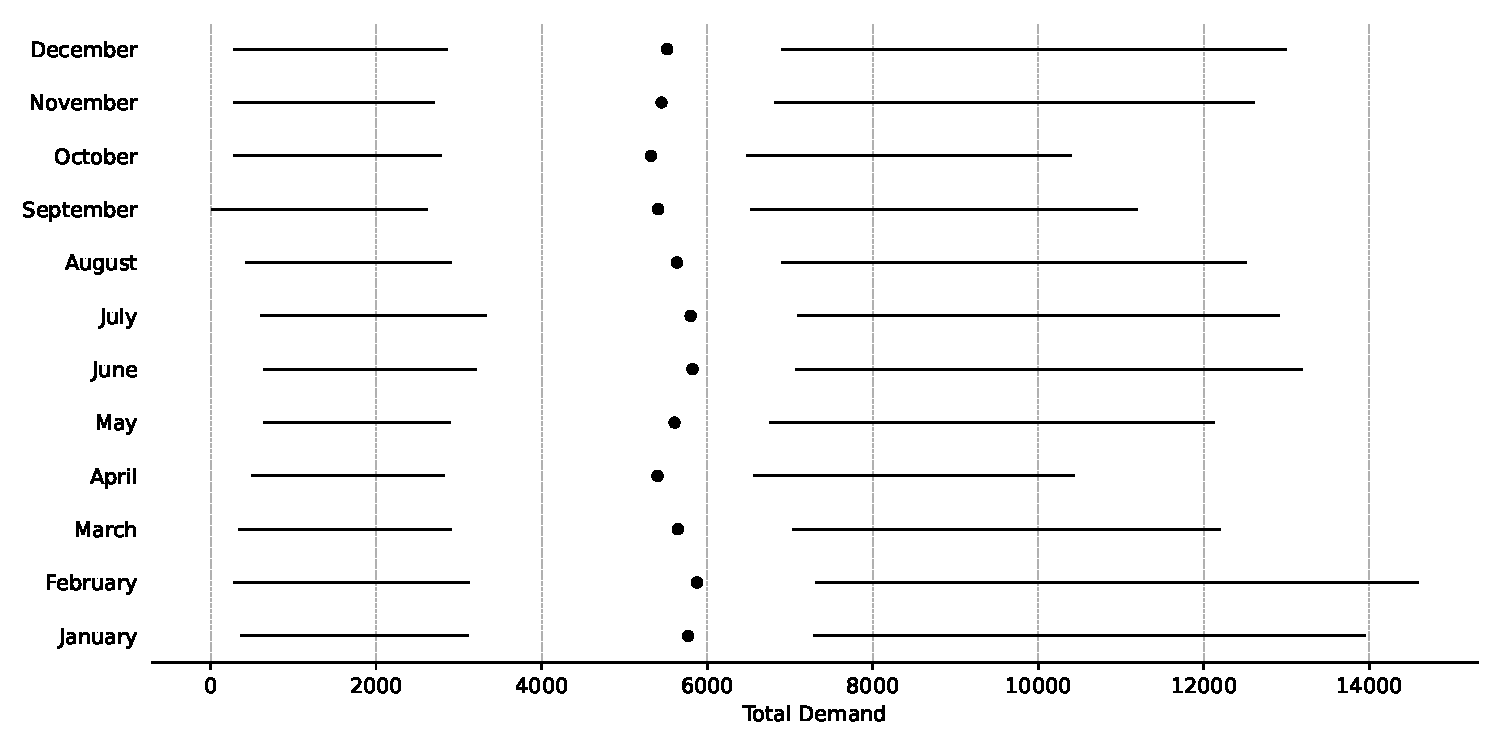
\includegraphics[width=\columnwidth]{Final Report/Figures/Plots/tufte_plot_month.pdf}}
\caption{Demand by Month Quartile Plot}
\label{tufte-plot-month}
\end{figure}

\begin{figure}[H]
\centerline{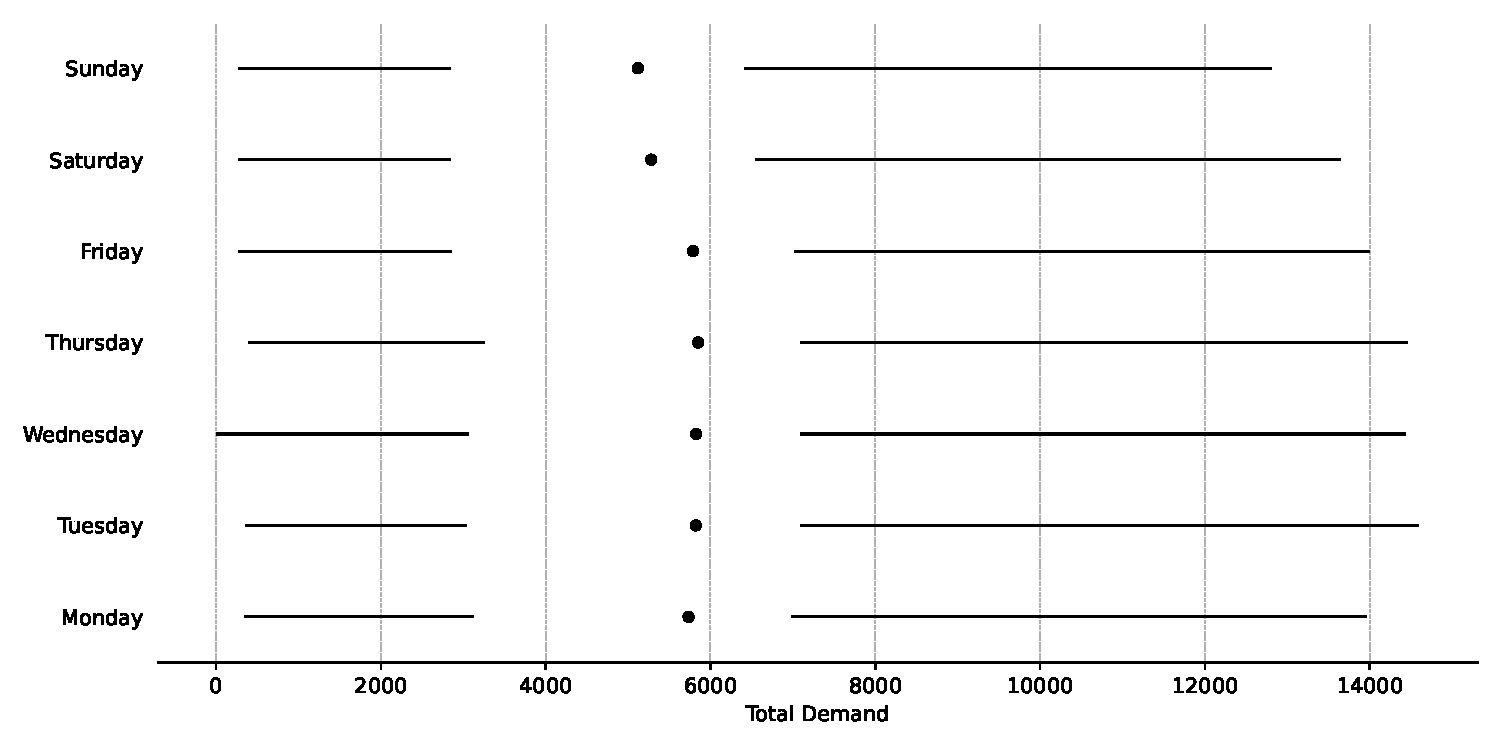
\includegraphics[width=\columnwidth]{Final Report/Figures/Plots/tufte_plot_day_of_week.pdf}}
\caption{Demand by Day of Week Quartile Plot}
\label{tufte-plot-weekday}
\end{figure}

Figure \ref{tufte-plot-month} shows a periodic correlation between the total demand and month of the year, which can again be attributed to increased heating and cooling in winter and summer. This correlation also demonstrates the value in performing the polar transformation described in Section \ref{transform-periodic}. In Figure \ref{tufte-plot-weekday}, there is an apparent increase in energy demand during the week and potentially a slight increase in mid-week demand.

\hypertarget{boolean-box-plots}{%
\section{Boolean Feature Box Plots}\label{boolean-box-plots}}

\begin{figure}[H]
\centerline{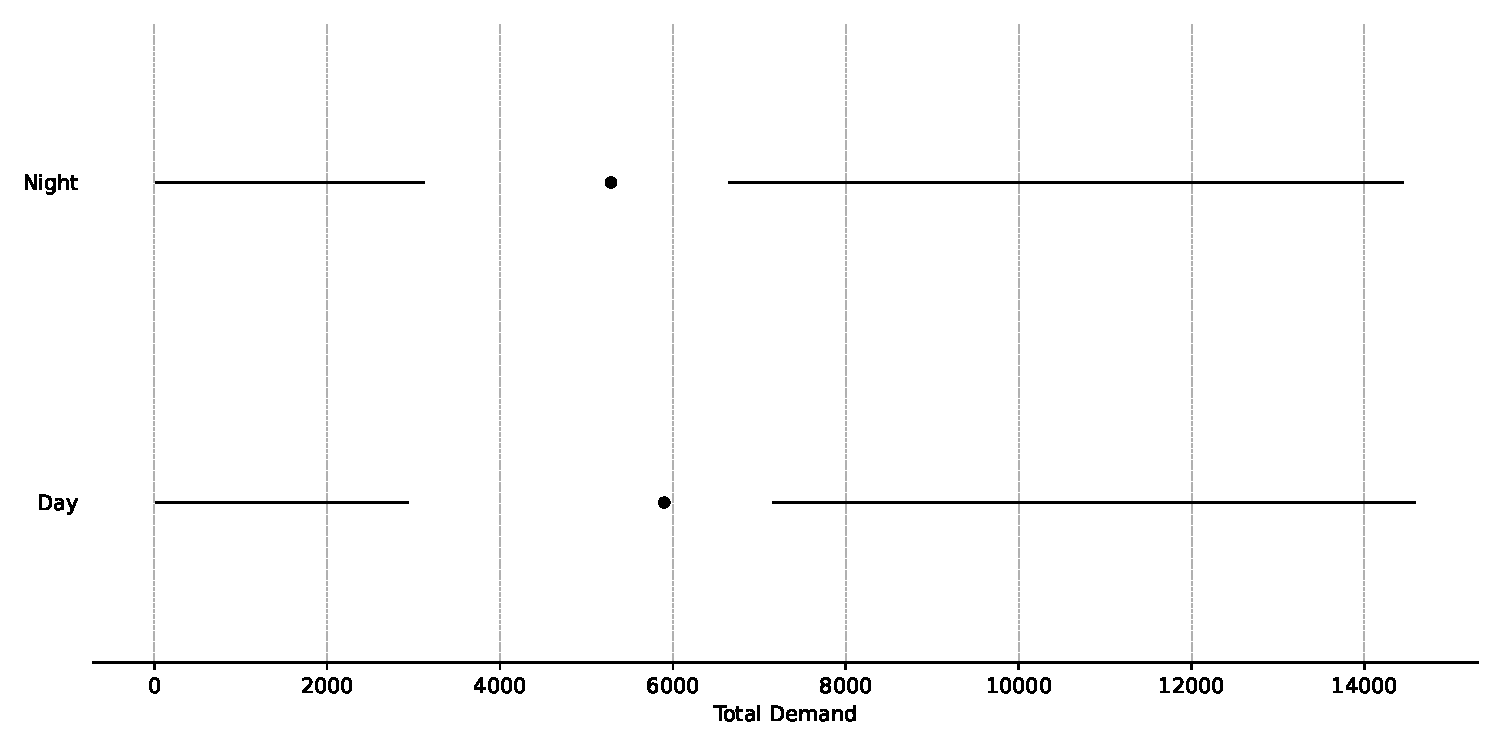
\includegraphics[width=\columnwidth]{Final Report/Figures/Plots/tufte_plot_is_daylight.pdf}}
\caption{Daylight Quartile Plot}
\label{tufte-plot-daylight}
\end{figure}

\begin{figure}[H]
\centerline{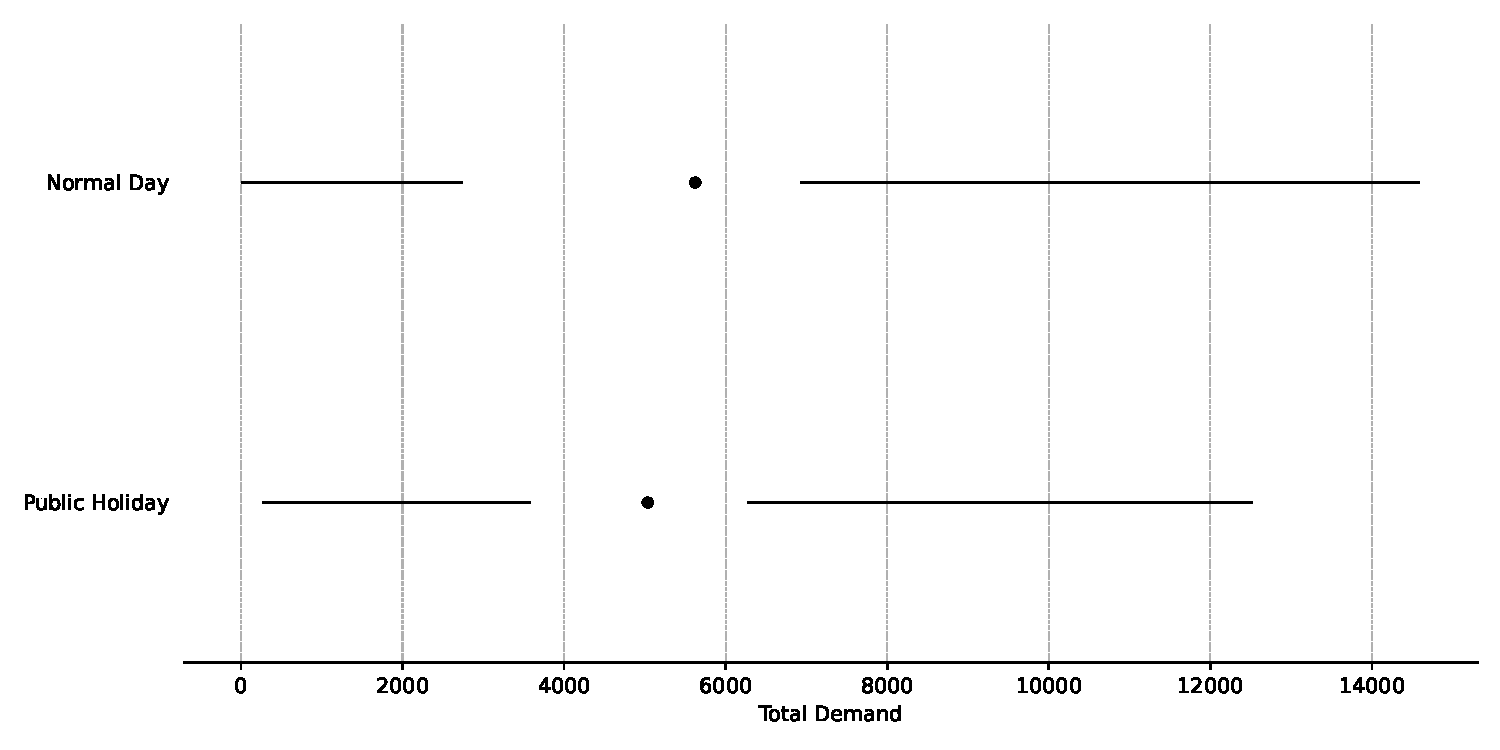
\includegraphics[width=\columnwidth]{Final Report/Figures/Plots/tufte_plot_is_public_holiday.pdf}}
\caption{Public Holiday Quartile Plot}
\label{tufte-plot-holiday}
\end{figure}

\begin{figure}[H]
\centerline{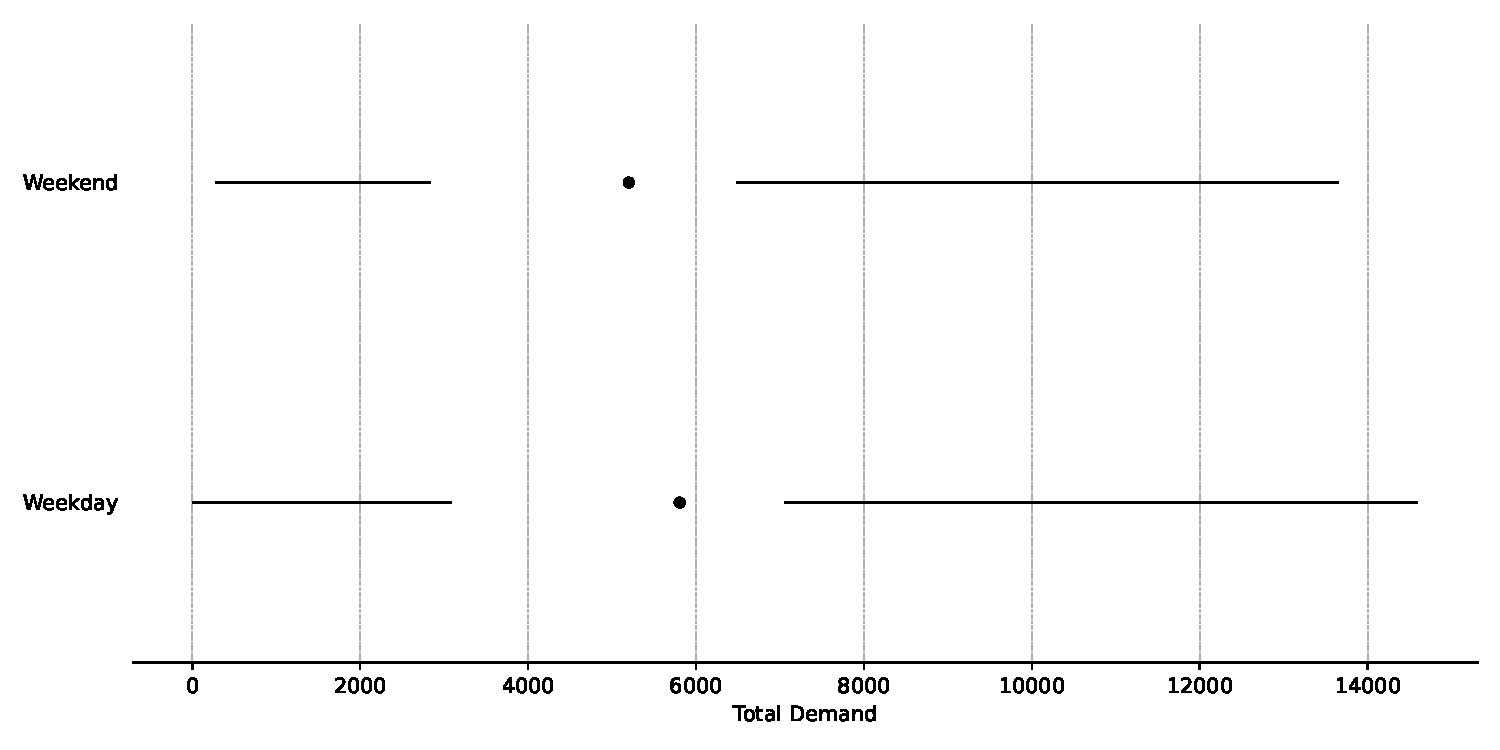
\includegraphics[width=\columnwidth]{Final Report/Figures/Plots/tufte_plot_is_weekday.pdf}}
\caption{Weekday Quartile Plot}
\label{tufte-plot-weekday}
\end{figure}

Figure \ref{tufte-plot-daylight} shows that whether there is daylight has a substantial impact on demand. This impact can be attributed to most of the population sleeping at night and, therefore, using less energy. \newline

Figure \ref{tufte-plot-holiday} shows that whether it is a public holiday strongly predicts total demand. Furthermore, given that it is binary, it can improve model accuracy with less computation required for training. It should also be noted that the spread (range and IQ range) on values is much smaller for public holidays since there are significantly less public holidays leading to variability uncertainty in the data.

\hypertarget{analysis-and-results}{%
\chapter{Analysis and Results}\label{analysis-and-results}}

\hypertarget{result-summary}{%
\section{Result Summary}\label{result-summary}}

We report the mean absolute percentage error (MAPE), the loss function of all models, and the root mean squared error (RMSE). When reviewing the basic ranking of the models (see Table \ref{mape-ranks}), we see that all MLP models outperformed all BD-LSTM (see Section \ref{learning-curve-analysis} for caveats). However, no broadly superior model is apparent from these results, as the univariate MLPs performed best on 1-hour-ahead forecasts, while the multivariate MLPs performed best on 24-hour-ahead forecasts. The competition between the models is further illustrated by the underlying MAPE results (see Table \ref{mape} and Figure \ref{mape_viz}). These illustrate that, although their batch-wise mean MAPEs are nearly indistinguishable, they perform substantially differently with different prediction horizons. Amongst the BD-LSTMs, the shallow multivariate model performs best, and the shallow univariate model performs worst. Between the deep BD-LSTMs, the multivariate model performed better on the 24-hour prediction horizon, and the univariate model performed marginally better on the one-hour prediction horizon.

A similar outcome is evident in the equivalent tables and visualisation for the test RMSE (Tables \ref{rmse-ranks} and \ref{rmse}; Figure \ref{rmse_viz}). Again, the multivariate MLPs perform best on 24-hour-ahead forecasts, and the univariate MLPs perform best on one-hour-ahead forecasts. However, the batch-wise means now place the multivariate MLPs as the best overall model on balance. Additionally, the univariate shallow BD-LSTM performs sufficiently well on this metric – especially on the 24-hour prediction horizon, where it places third – to place fourth overall. The deep multivariate BD-LSTM outperforms both univariate LSTMs on all aspects of RMSE.

The success of the MLPs as a category is also seen in Table \ref{model-group-MAPE}. Here, we can see that the MLPs' mean MAPE is superior to the BD-LSTMs' by both prediction horizons and their mean. Table \ref{complexity-MAPE} shows that the shallow models performed marginally better than the deep models by both prediction horizons and their mean. Table \ref{input-type-MAPE} shows that the multivariate models outperformed the univariate models overall, but the univariate models did perform marginally better on the 24-hour prediction horizon. Identical patterns are borne out by the aggregated mean RMSEs in Tables \ref{model-group-RMSE}, \ref{complexity-RMSE}, and \ref{input-type-RMSE}.

\CatchFileDef{\mape-ranks}{Tables/model MAPE ranks.tex}{} \mape-ranks
\CatchFileDef{\mape}{Tables/model MAPEs.tex}{} \mape

\begin{figure}[H]
\centerline{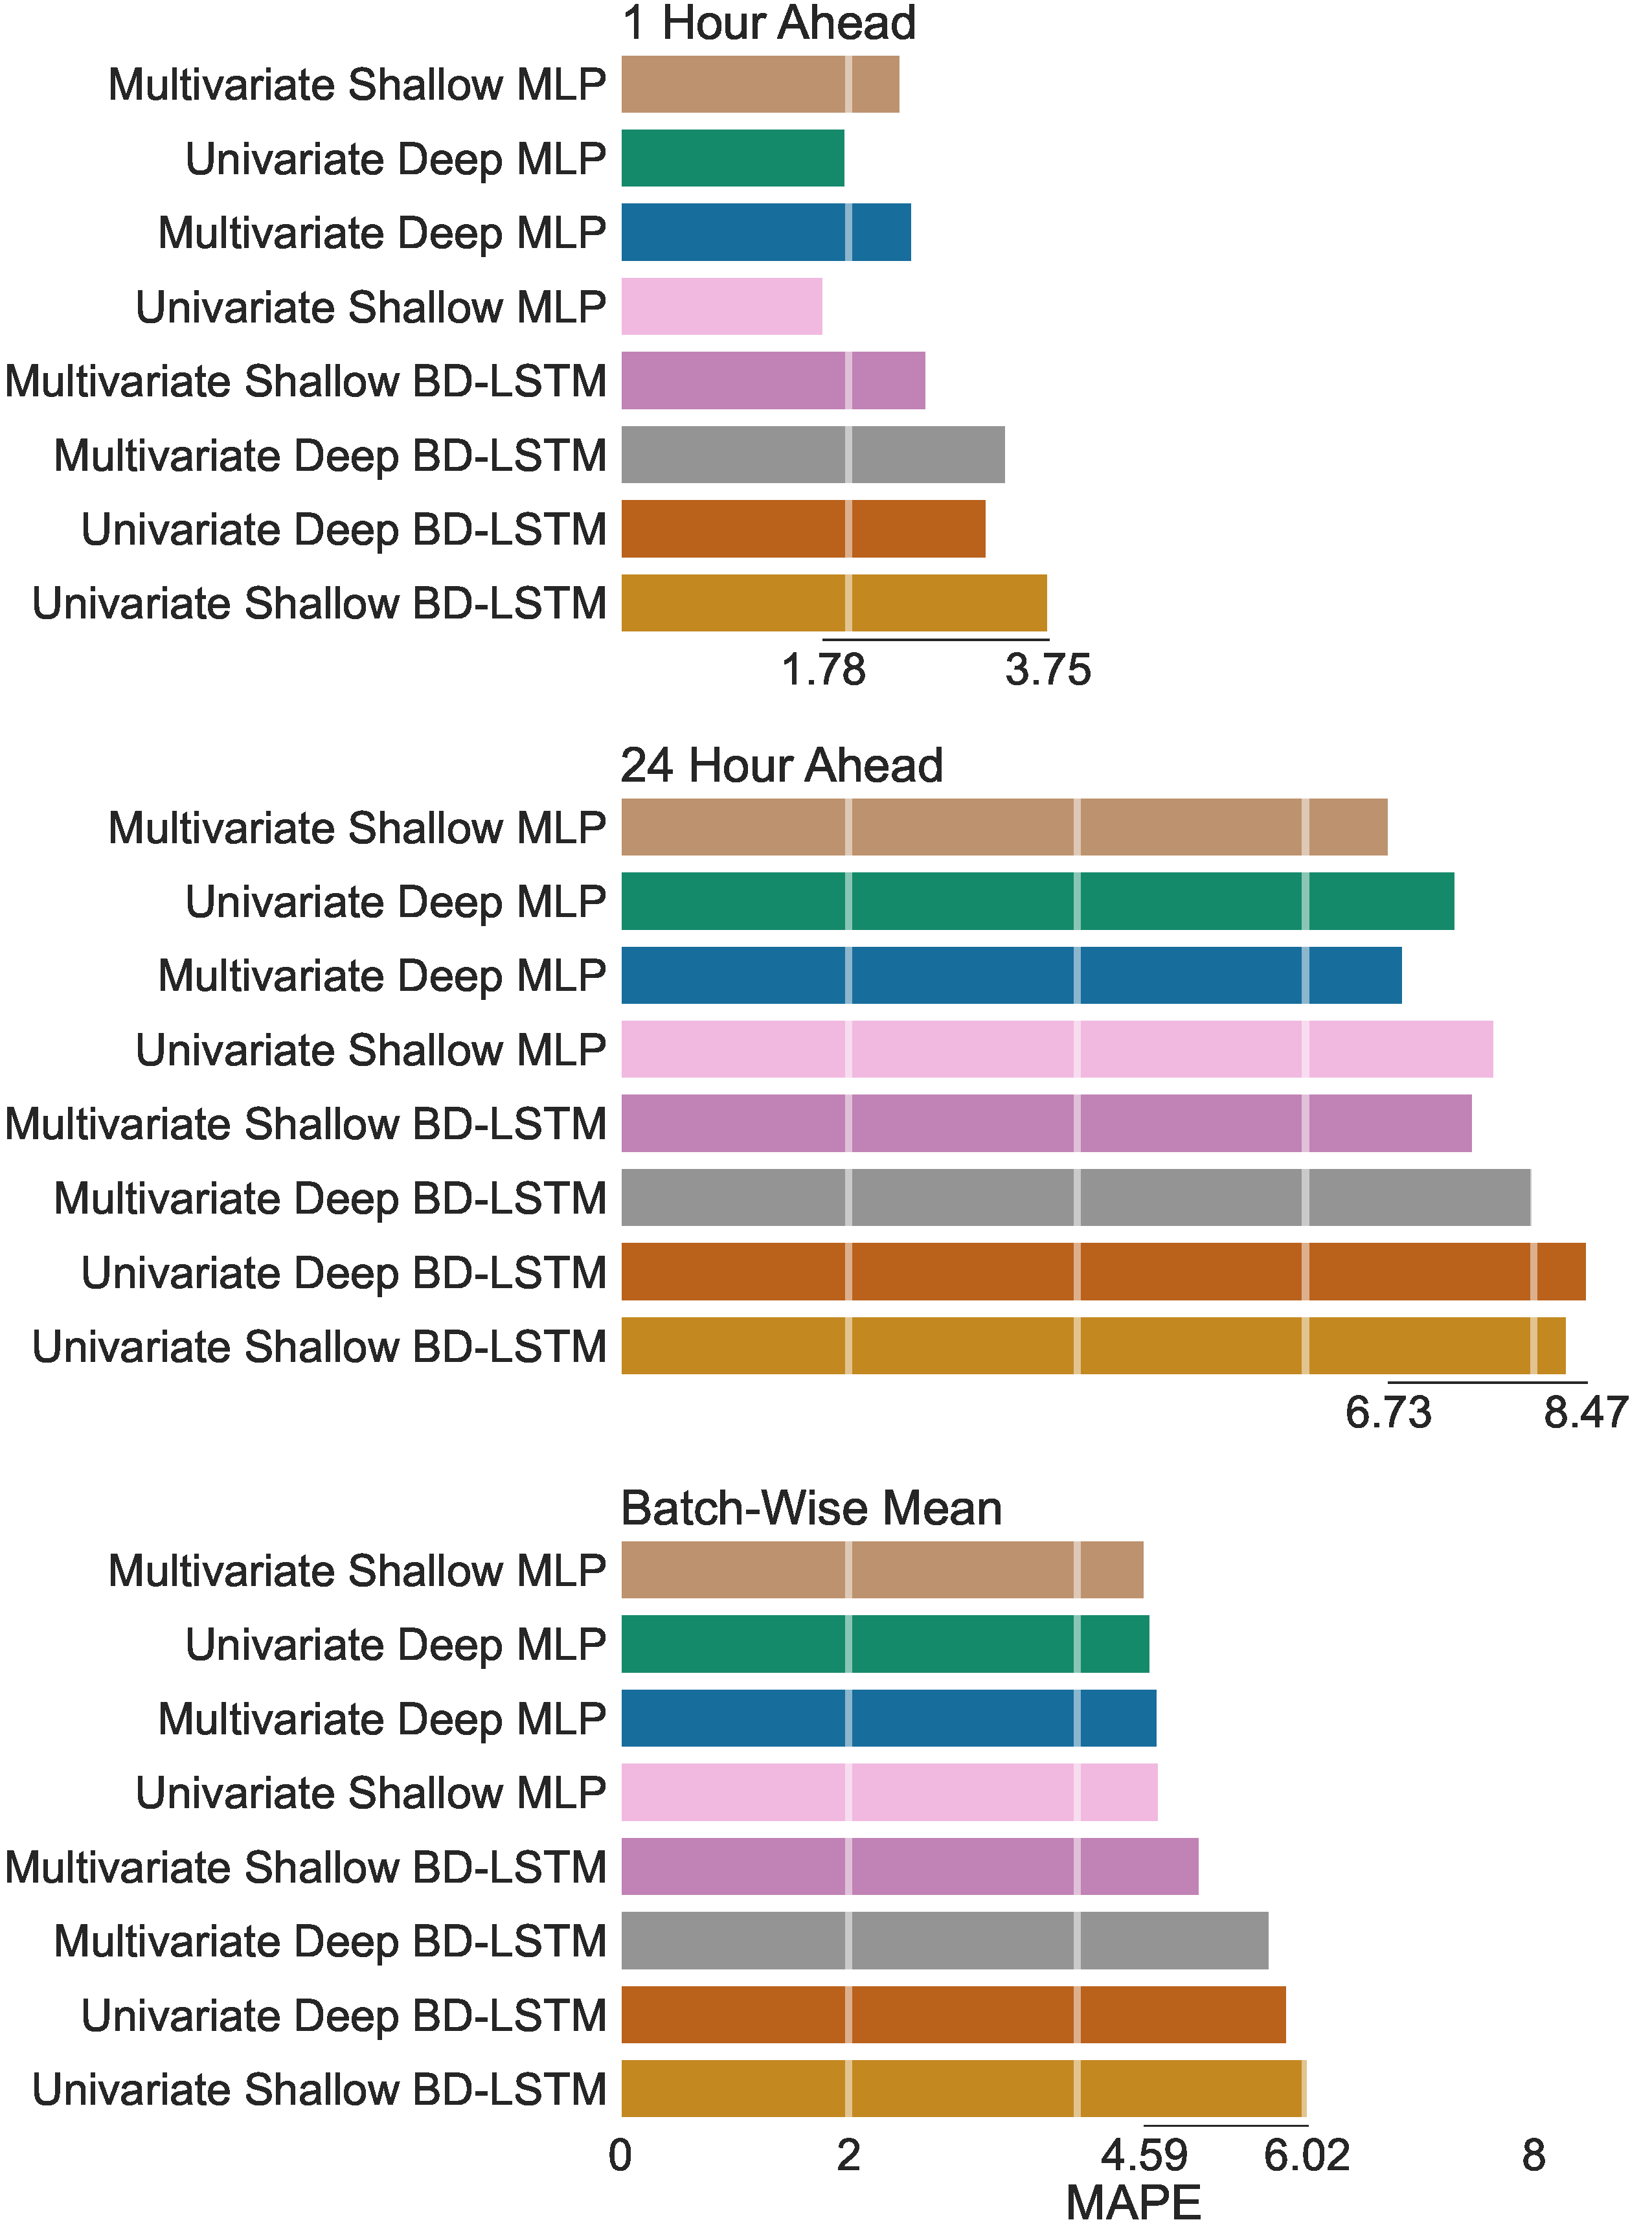
\includegraphics[width=\columnwidth]{Figures/Plots/Test MAPE results.pdf}}
\caption{Horizontal bar charts with range frames showing the MAPE test results for the eight models. The tests covered the one- and 24-hour ahead prediction horizons and their batch-wise mean. The models are ordered by the mean.}
\label{mape_viz}
\end{figure}

\CatchFileDef{\rmse-ranks}{Tables/model RMSE ranks.tex}{} \rmse-ranks
\newline
\CatchFileDef{\rmse}{Tables/model RMSEs.tex}{} \rmse

\begin{figure}[H]
\centerline{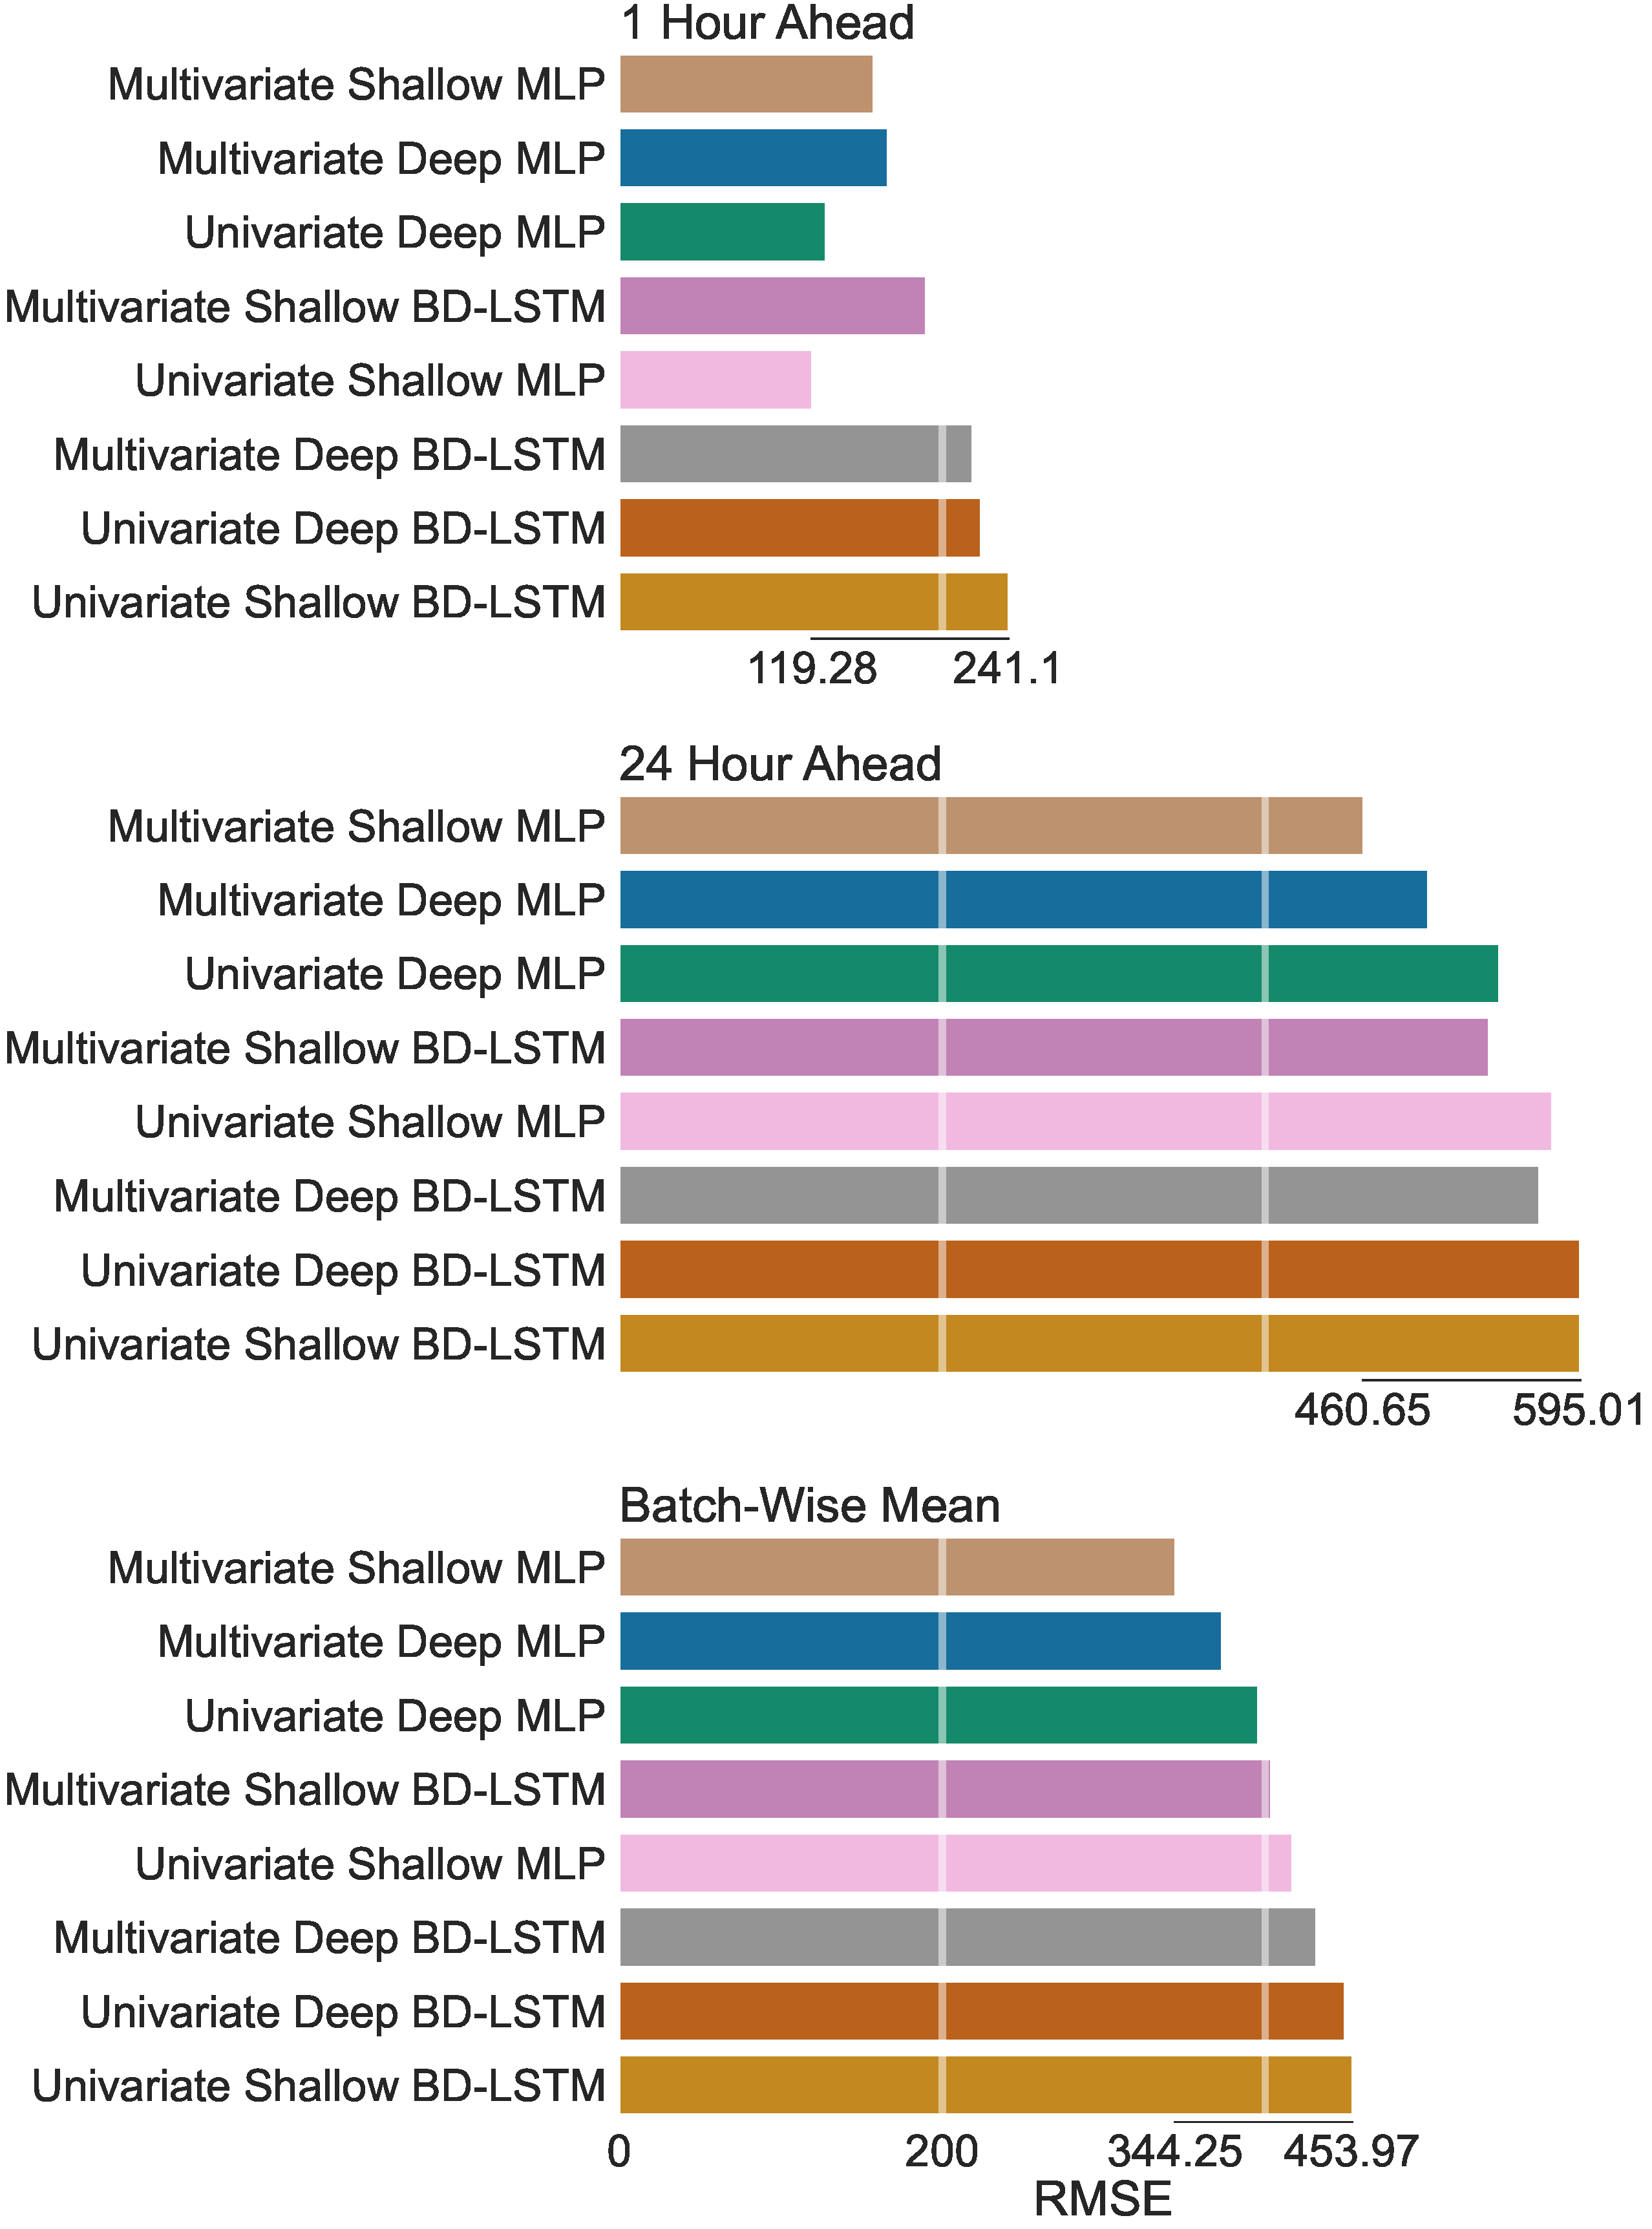
\includegraphics[width=\columnwidth]{Figures/Plots/Test RMSE results.pdf}}
\caption{Horizontal bar charts with range frames showing the RMSE test results for the eight models. The tests covered the one- and 24-hour ahead prediction horizons and their batch-wise mean. The models are ordered by the mean.}
\label{rmse_viz}
\end{figure}

\CatchFileDef{\model-group-MAPE}{Tables/MAPE grouped by model group.tex}{} \model-group-MAPE
\CatchFileDef{\model-group-RMSE}{Tables/RMSE grouped by model group.tex}{} \model-group-RMSE
\CatchFileDef{\complexity-MAPE}{Tables/MAPE grouped by complexity.tex}{} \complexity-MAPE
\CatchFileDef{\complexity-RMSE}{Tables/RMSE grouped by complexity.tex}{} \complexity-RMSE
\CatchFileDef{\input-type-MAPE}{Tables/MAPE grouped by input type.tex}{} \input-type-MAPE
\CatchFileDef{\input-type-RMSE}{Tables/RMSE grouped by input type.tex}{} \input-type-RMSE



\hypertarget{learning-curve-analysis}{%
\section{Learning Curve Analysis}\label{learning-curve-analysis}}

The learning curves of the MLPs (Figure \ref{mlp_hists}) overall show that the models fit the data well. The exception is the deep multivariate model: its comparatively chaotic test curve is unusual. Instability in the test curve could result from an insufficiently large test set. However, the test set was enormous. This hypothesis would also fail to explain the instability in the train curve. We hypothesise that this has resulted from the learning rate scheduling. The larger learning rate in the schedule may have been too great, such that it deteriorated the coefficients much of the time. Additionally, both the train and test values were decreasing when the training stopped, indicating that this model may be underfitting the data. Additional training would improve this. Another point of potential concern for model misspecification is that the test MAPE of the multivariate shallow MLP increases for the final 8000-9000 epochs. However, as the models only saved the weights of the iteration performing best on the test set, the final model tested would not suffer from the overfitting evident in this plot.

The learning curves of the BD-LSTMs (Figure \ref{lstm_hists}) show that the models are generally, if not entirely, underfitting the data. A well-fitted model will decrease its loss function rapidly before the loss largely stabilises, and it may gradually improve after that point for a large number of epochs. None of these models could have undergone the gradual improvements, and it is unclear that the univariate deep model has completed the initial stabilisation. Subsequently, the ranking and comparisons made in Section \ref{result-summary} are, at best, inconclusive. However, given that the train and test curves move in tandem, the models do not show signs of more pervasive underfitting or overfitting. As such, additional training should be sufficient to correct the underfitting present and make meaningful comparisons between the models \cite{Ng2018}.

Figures \ref{mlp_hists} and \ref{lstm_hists}, at least tentatively, also show that all models are substantially biased compared to the AEMO Market Management System forecasts. Although we cannot be sure that further training of the LSTM and multivariate deep MLP models would not result in substantial improvements in the loss, the results of this study do not make that outcome appear likely. Further research and experimentation would likely be needed to improve upon AEMO's model. 

\begin{figure}[H]
\centerline{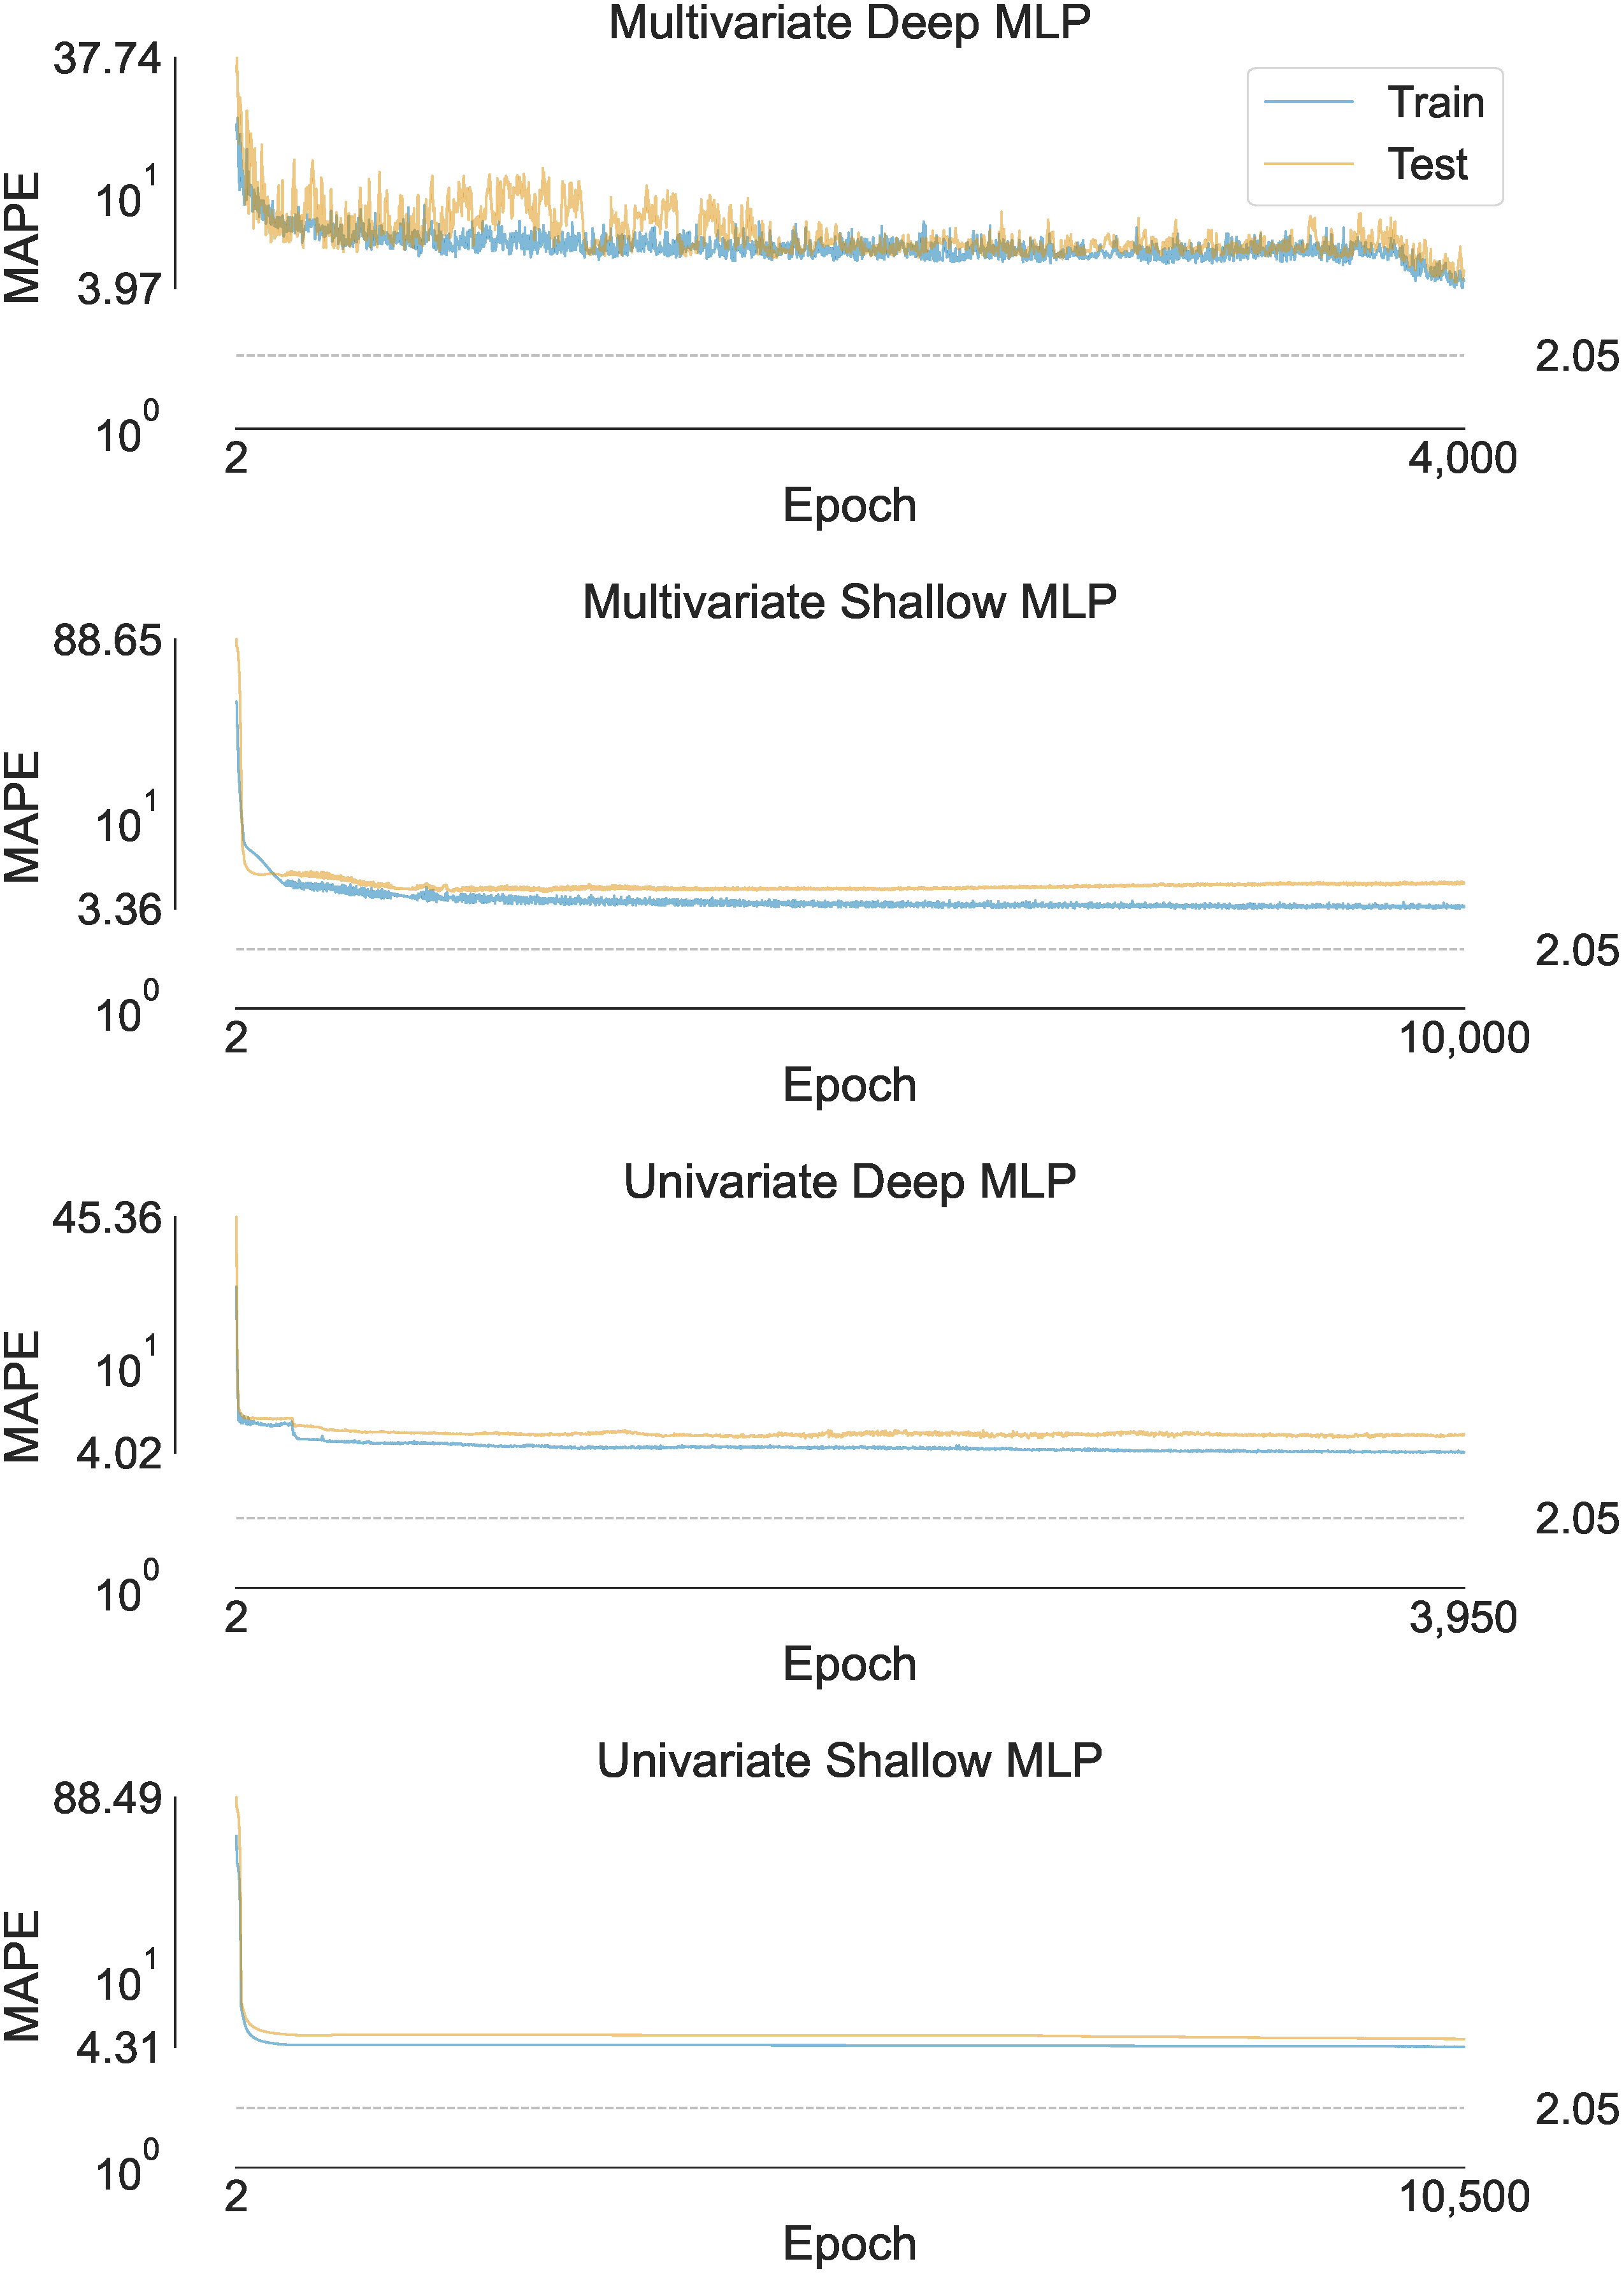
\includegraphics[width=\columnwidth]{Figures/Plots/MLP training histories.pdf}}
\caption{Training histories for each MLP showing the training and test loss (MAPE) by epoch of training. Only even epochs are shown, as the learning rate scheduling makes the full history appear noisier than it is. The dotted line represents the equivalent MAPE of the AEMO Market Management System model. The y-axis has a logarithmic scale.}
\label{mlp_hists}
\end{figure}

\begin{figure}[H]
\centerline{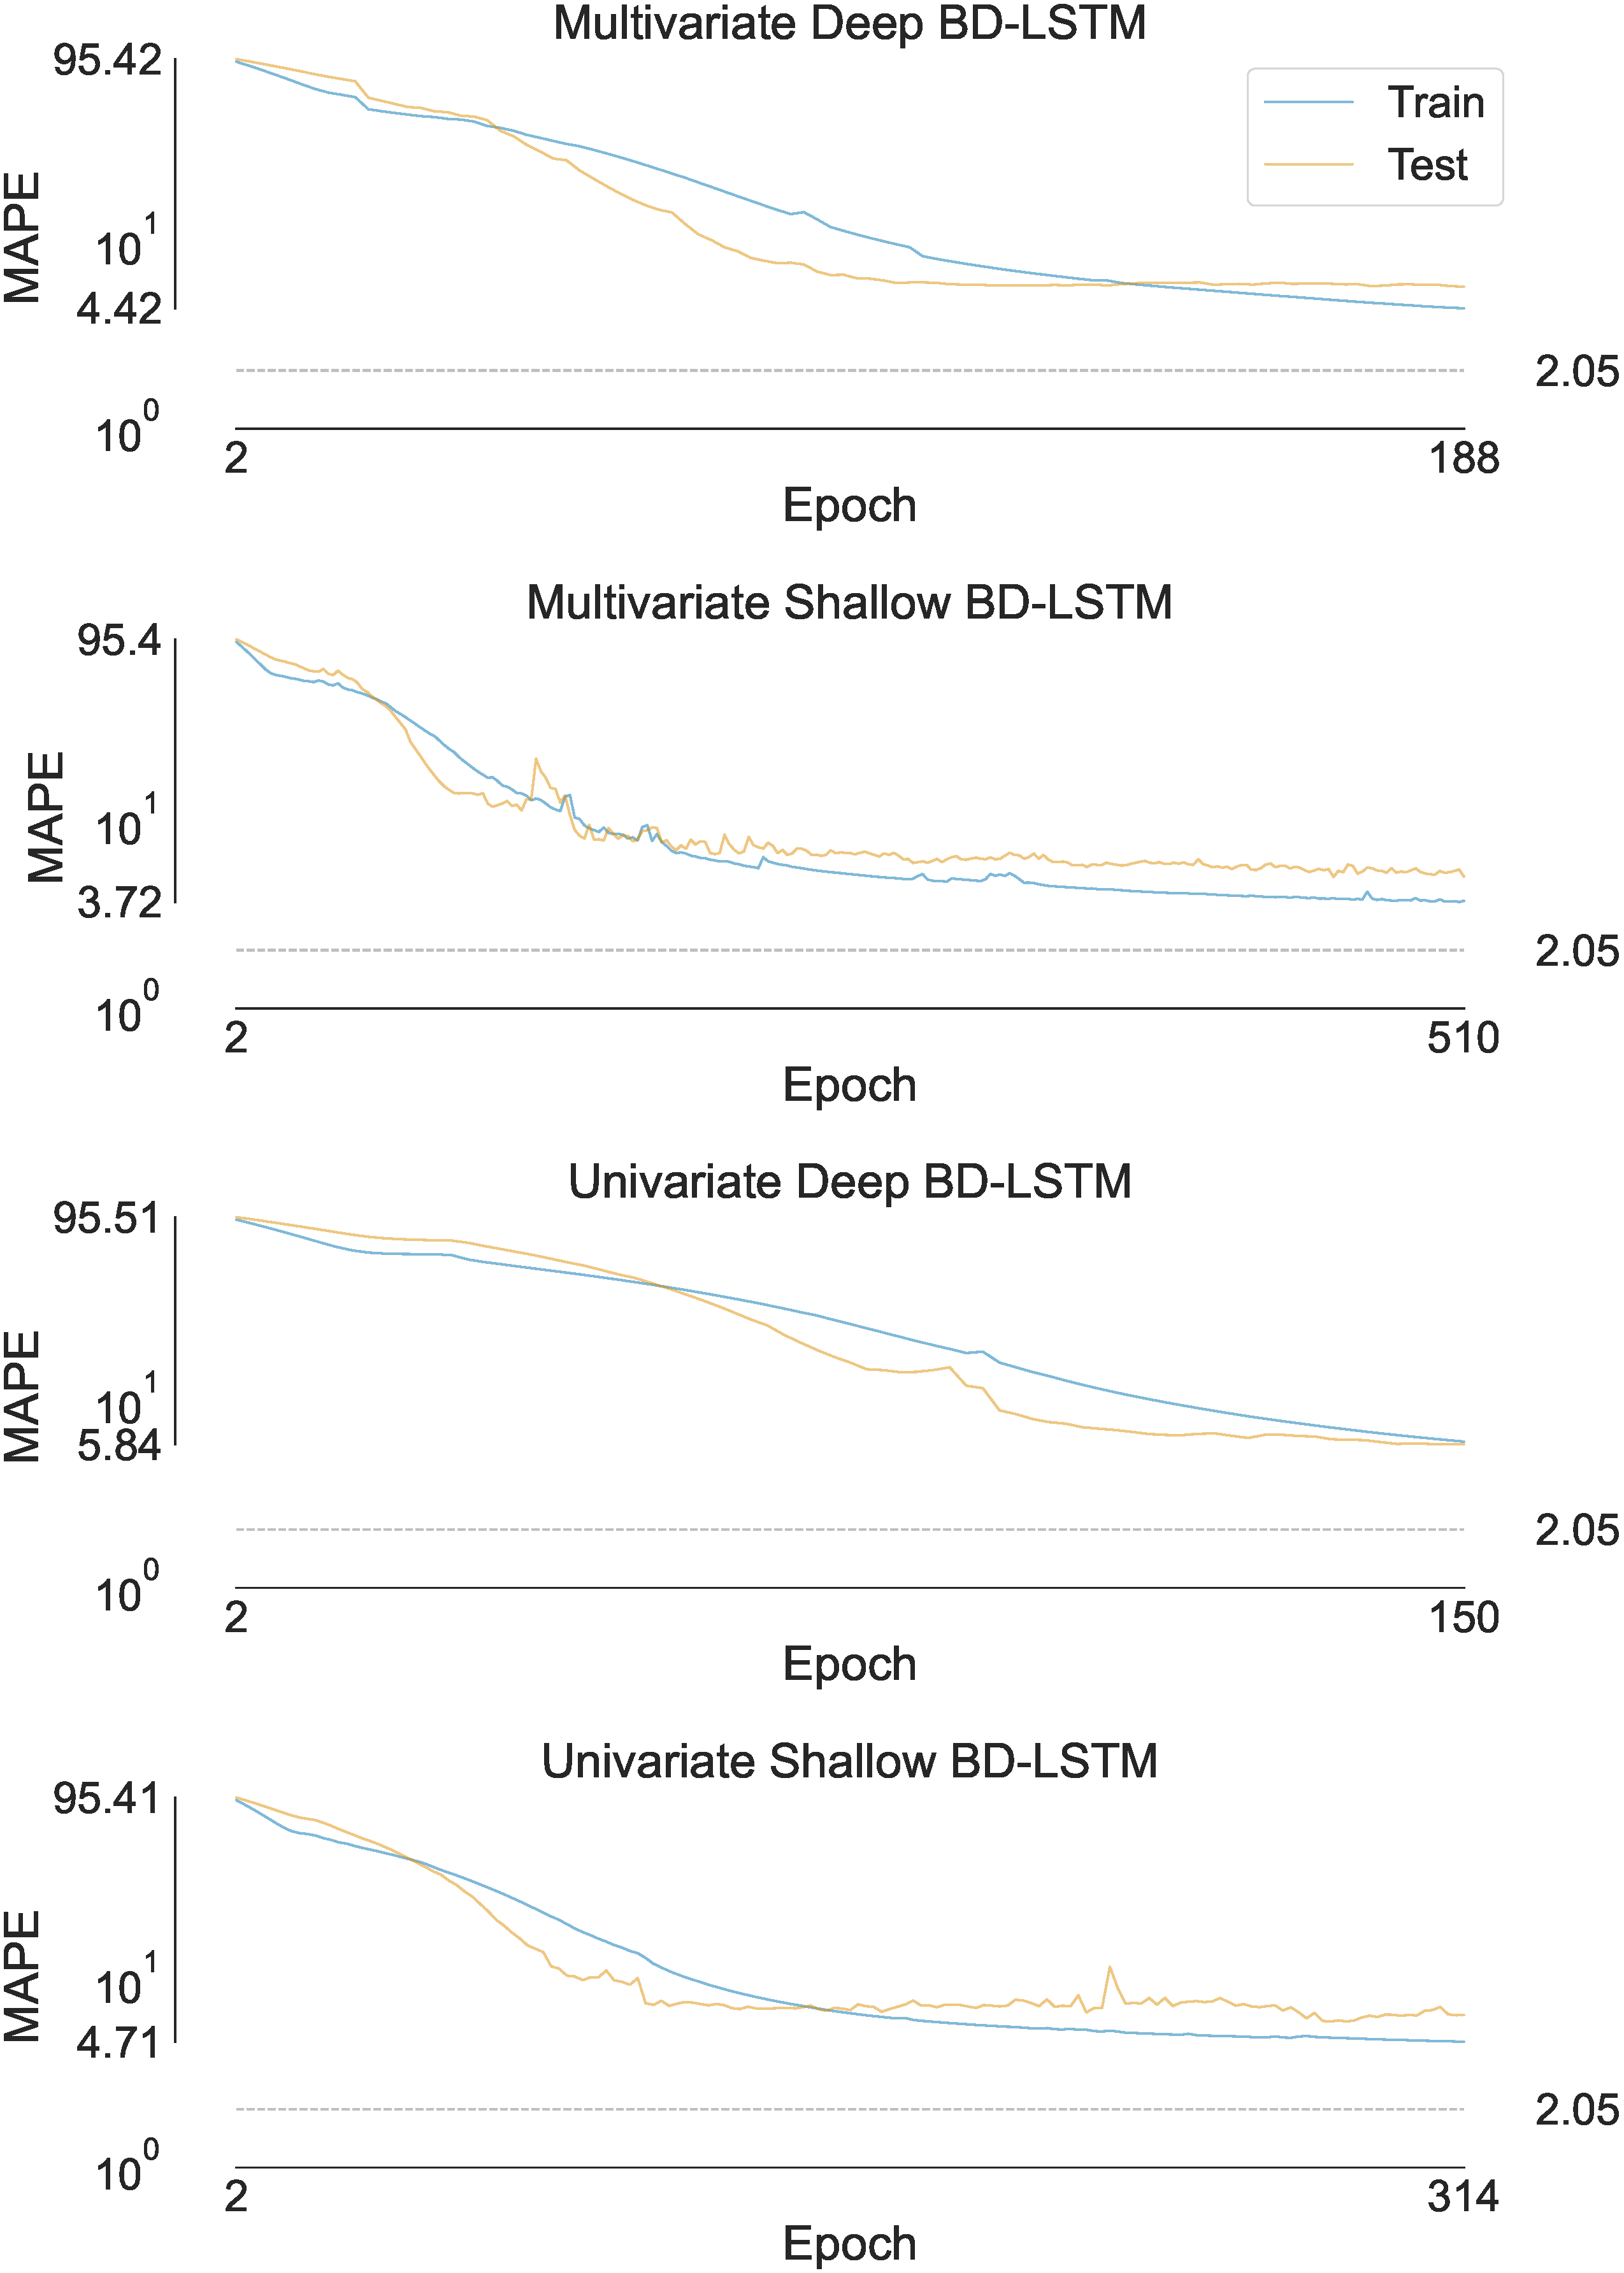
\includegraphics[width=\columnwidth]{Figures/Plots/BD-LSTM training histories.pdf}}
\caption{Training histories for each BD-LSTM showing the training and test loss (MAPE) by epoch of training. Only even epochs are shown, as the learning rate scheduling makes the full history appear noisier than it is. The dotted line represents the equivalent MAPE of the AEMO Market Management System model. The y-axis has a logarithmic scale.}
\label{lstm_hists}
\end{figure}


\hypertarget{discussion}{%
\chapter{Discussion}\label{discussion}}

% Put the results you got in the previous chapter in perspective with
% respect to the problem studied.
The performance results for the eight models tested are given in Tables \ref{mape} and \ref{rmse}. The MLPs performed markedly better than the BD-LSTMs, with all MLPs outperforming all BD-LSTMs by the mean metric, with the one exception of the multivariate shallow BD-LSTM having a lower mean RMSE than the univariate shallow MLP. At first glance, this is surprising, given the added complexity of the BD-LSTM networks, with their recurrent layer designed to capture long-term dependencies in time-series data, compared to a feed-forward MLP. If we examine the loss curves in Figure \ref{lstm_hists}, we see that, for the BD-LSTM networks, the curves were only just approaching stabilisation, particularly for the deep networks, and still had the potential to improve given more training time. The MLP networks, alternatively, had stabilised early in the training and easily reached their peak performance. Had more time been available to train these models, based on the research surveyed in Chapter \ref{literature-review}, we would expect the BD-LSTM to outperform the MLP networks. The time constraint of this project is therefore a defining factor in the outcome of the comparison between model architectures. However, many other conclusions can be drawn. 

In particular, the increased computational load imposed by using deep and complex NN models dramatically affects training time. This effect is demonstrated in Table \ref{ttimes}, which shows that in a similar time period of around two hours, the most complex model (the multivariate deep BD-LSTM) was only able to complete 21 epochs, whereas the simplest model (the univariate shallow MLP) was able to complete 10,500. The former model was run for 189 epochs in this study over nearly ten hours, and while it continued to show signs of improvement when training ceased, ultimately, it was outperformed by the simpler model on nearly all metrics\footnote{The single exception to this is that the multivariate shallow BD-LSTM had a marginally lower RMSE on 24-hour-ahead forecasts than the univariate shallow MLP}. In fact, the simple model performed best out of all models for the 1-hour-ahead prediction, with a MAPE of 1.78 and an RMSE of 119.28, compared to the multivariate deep BD-LSTM which ranked 6th for 1-hour-ahead predictions, with MAPE of 3.38 and RMSE of 218.85. 

Apart from more training time, another improvement that could contribute to the inherent advantage of more complex models is additional time for hyperparameter tuning and testing of model configuration. With time being a significant constraint, a compromise had to be made when selecting hyperparameters, with a grid search performed on the shallow version of each network and the results applied to both shallow and deep networks. Consequently, each model was not optimised. Ideally, each model architecture should have its own set of hyperparameters that were determined by more sophisticated means, as outlined in Chapter \ref{literature-review}. An optimised architecture and hyperparameter set may have helped to get the most out of the BD-LSTM models.

Tables \ref{mape} and \ref{rmse} show that in three out of the four model pairs, the multivariate model outperformed the univariate model, on average, in terms of both MAPE and RMSE. The exception was the deep MLP, where the average MAPE for the univariate case was slightly better (4.64 compared to 4.70). However, for the RMSE, the reverse was true: 395.71 compared to 373.06. So, in general, we have shown that multivariate models have outperformed their univariate equivalents (with the same architecture and hyperparameters). We expected this outcome, as more information is being fed into the models, allowing them to learn more complex relationships between attributes. The downside of adding more features is the increase in training time, as evident in Table \ref{ttimes}. However, this effect was far more pronounced in the BD-LSTM variants than for the MLPs, where the differences were marginal.

Comparing the NN pairs by complexity (i.e. shallow vs. deep network), the results were inconclusive as to whether a deeper architecture is likely to provide higher accuracy. In both multivariate pairs (MLP and BD-LSTM), the shallow network outperformed the deep network, on average. While most differences between pairings were small, the multivariate BD-LSTM pair had the most significant difference in performance, with the shallow network's MAPE average being 5.07, compared to the deep network's 5.68. In both univariate pairs, the deep networks performed better. With the MLP networks able to train long enough to reach their optimal performance, we can conclude that, for the chosen architectures and hyperparameters, there is no clear advantage to increasing model depth. The computationally expensive BD-LSTM networks required more training time to reach their optimal performance, especially the deep variant. As such, no definitive conclusion can be drawn from these results.

Another factor that has impacted results is the differing load profiles over each state, seen in Figure \ref{demand-distributions-plot}. Combining the datasets from each state has resulted in more generalised models, but models may be improved by training only on data specific to each state. We recommend that state-specific models be tested and compared to the general case. Further, our imputation method was insufficiently robust to handle large stretches of missing data from the Victorian dataset. Issues with imputation resulted in a large cluster of values skewing the results. Better imputation should be implemented in future tests.

Further improvements could come from more sophisticated temperature or weather data use. While the electrical load data was supplied for the entirety of each state, the temperature observations are from a single station in each state and may not be representative of the temperature across large and varying Australian states and their climates. It is recommended that temperature data across all weather stations be obtained and an average temperature value be used, possibly weighted by population density around each weather station, as electrical load heavily correlates with population.

Additionally, the relatively biased results presented here were surprising, given the results seen as we designed the models. This disparity between expectation and outcome may partly result from overfitting the training and validation data. However, we hypothesise that there would be additional benefits to training one model per state. Given that Australia is large and includes multiple climatic regions, it is plausible that the data used in this report and its patterns vary more across states than our models could manage. Future research could review whether one model per state or climatic region provides greater accuracy than one model for all regions.


\hypertarget{conclusion-and-further-issues}{%
\chapter{Conclusion and Further
Issues}\label{conclusion-and-further-issues}}

Overall, we recommend further testing to optimise the BD-LSTM networks and ensuring sufficient training time to obtain results in line with the research outlined in Chapter \ref{literature-review}. It remains plausible that these changes would create a model superior to the AEMO Market Management System model. It would also be worth further investigating and comparing the performance of a 1D-CNN model, a relatively new approach to STLF that has shown promise, and a GRU, commonly used for this kind of task. With that said, good performance was able to be achieved using very simple NN architecture, with the top performing model, on average, being the multivariate shallow MLP.

This study has shown that multivariate modelling has an advantage, that the addition of more exogenous variables, such as solar radiance, wind, and solar panel uptake, could enhance model accuracy, and that the feature engineering implemented was worthwhile.

We could not draw a clear conclusion regarding the potential advantage of increasing model depth, as our results on this were mixed. However, deeper models require more training time, and the models presented here may have fallen substantially below their full potential in this test due to time constraints. The BD-LSTM cases, in particular, could improve with lesser time constraints. More work should be done to investigate this matter.

While training time is an essential factor to consider and a major differentiator between the models compared in this study, it is time that only needs to be spent in the development phase. Once the model is trained, it can be implemented without significant additional cost. Therefore the model producing the best prediction accuracy should be chosen, providing it can be tuned and trained within the client's time frame.

\bibliographystyle{elsarticle-num}
\bibliography{references}

\hypertarget{appendices}{%
\chapter*{Appendices}\label{appendix}}
\addcontentsline{toc}{chapter}{Appendices}

\renewcommand*\thesection{A.\arabic{section}} % Number appendices starting at A.1.

\hypertarget{code}{\section{Code}\label{code}}

This project was managed through \textit{GitHub}. Our code and more information about our work can be found at \href{https://github.com/mango-unchained/Team-K---ZZSC9020-Capstone-Project}{Team K ZZSC9020 Capstone Project}.

\hypertarget{data}{\section{Data}\label{data}}

\renewcommand*\thetable{A.\arabic{table}} % Number tables starting
\renewcommand*\thefigure{A.\arabic{figure}} % Number tables starting

\begin{figure}[H]
\centerline{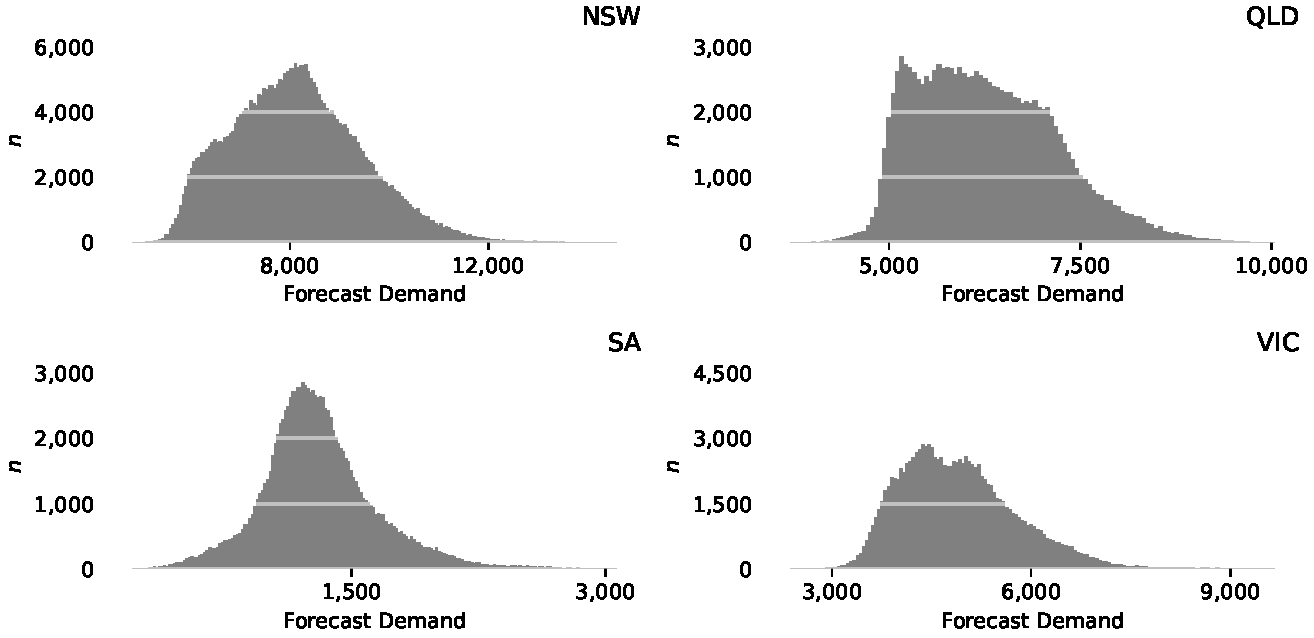
\includegraphics[width=0.8\columnwidth]{Final Report/Figures/Plots/Forecast demand histogram.pdf}}
\caption{A histogram of forecasted demand for NSW.}
\label{fdemand}
\end{figure}

\begin{figure}[H]
\centerline{\includegraphics[width=\columnwidth]{Final Report/Figures/Plots/Forecast vs. actual for 1- and 24-hours.png}}
\caption{Scatter plots of forecast vs. total demand for NSW. The one-hour-ahead (i.e. two-periods-ahead) correlation appears on the left, and the one-day-ahead correlation appears on the right.}
\label{fdemand_vs_tdemand}
\end{figure}

\begin{figure}[H]
\centerline{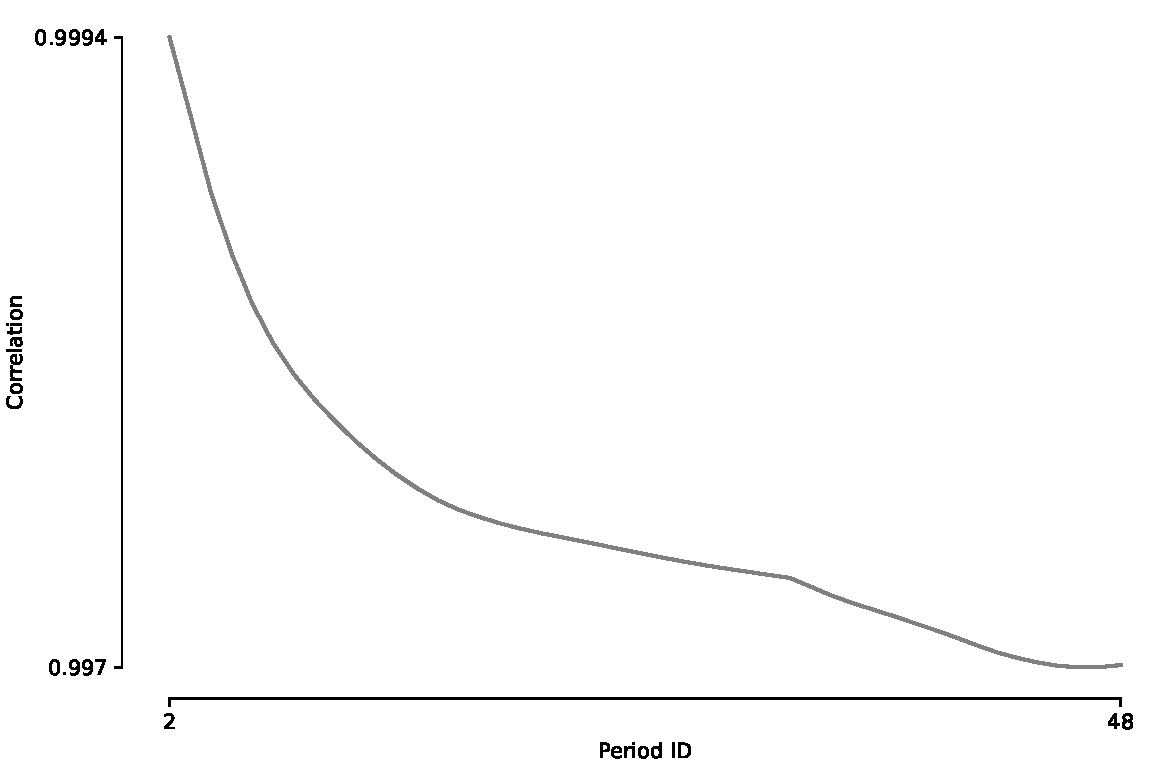
\includegraphics[width=0.8\columnwidth]{Final Report/Figures/Plots/Forecast vs. actual correlation by Period ID.pdf}}
\caption{A line plot of the Pearson correlation coefficient of forecast and total demand vs. the period ID. Each period represents a thirty-minute interval. As such, the X-axis also represents the correlations from one-hour-ahead to one-day-ahead forecasts.}
\label{corr_by_per}
\end{figure}

\begin{landscape}
\hypertarget{appendix-preprocessing-pipeline}{\section{Pre-processing Pipeline}\label{appendix-preprocessing-pipeline}}

\begin{figure}[H]
    \centering
    \includegraphics[width=\linewidth]{"Final Report/Figures/feature_engineering.png"}
    \caption{Feature Engineering Pipeline.}
    \label{feature-engineering-process}
\end{figure}

\end{landscape}

\end{document}

